% Autoř: Vladyslava Bilyk(xbilyk03)

\chapter{Úvod}
\label{ch:1}
V dnešní době je množství webových stránek, článků a dalších věcí na internetu tak velké, že život člověka nestačí na to, aby vše prošel. Na internetu najdete nejrůznější informace a širokou škálu společností a produktů, které dodávají. A to není omezeno na zemi, kde se člověk nachází. World Wide Web pokrývá téměř všechny části našeho světa. Protože najít a vybrat si z velkého množství nabízených služeb tu správnou je obtížný úkol, uživatelé se obvykle spoléhají na hodnocení a reklamu. Chcete-li propagovat svůj produkt, musíte o něm dát lidem vědět, a proto se reklama stala nedílnou součástí našeho života. Každý den se s ní uživatelé setkávají nejen na ulici, ale také online. Prohlížeče, webové stránky a aplikace jsou plné nejrůznějších reklam.

Společnosti se snaží najít co nejefektivnější způsoby propagace svých výrobků. Pokud se jedná o velkou společnost, je také důležité optimalizovat práci reklamní kampaně. K tomuto účelu se používají analytické, marketingové a remarketingové skripty. Shromažďují~informace o akcích uživatelů na stránce -- kolik lidí se zaregistrovalo, kolik jich navštívilo tu~či onu stránku, kolik kliknutí bylo provedeno na tomto formuláři, kolik lidí si koupilo tento produkt, kolik jich opustilo stránku ve fázi objednávky atd. Všechny tyto informace jsou užitečné při nastavování reklamní kampaně~\cite{analitic}.

Než se uživatel stane klientem společnosti, projde několika fázemi interakce s webovou stránkou. Od kliknutí na reklamní banner přes seznámení se s produktem až po zájem o společnost. Těmito fázemi projde každý uživatel, který navštíví webové stránky, ale ne každý dosáhne té poslední -- stane se stálým zákazníkem~\cite{funnel}.

V počáteční fázi se hodí marketingové skripty, které pomohou společnostem neztratit potenciální návštěvníky a povzbudit nové. Když je uživatel na webu, analytický skript aktivně pracuje a shromažďuje informace, poté je převede do zpráv. Remarketingové skripty se hojně využívají k návratu návštěvníků, kteří web bez zájmu opustili. Každý skript nabízí široké možnosti a různé varianty použití. Můžete je konfigurovat a integrovat do kódu pomocí nástrojů, které poskytují služby svým klientům. Mezi příklady takových nástrojů patří Google Analytics~\cite{accountA} a Google Ads~\cite{accountM}.

Bohužel ne vždy se reklama, sledování uživatelů a další skripty používají v souladu s právními předpisy. I když existuje nařízení Evropské unie, konkrétně obecné nařízení o ochraně osobních údajů, zkráceně GDPR~\cite{GDPR}, které chrání důvěrná práva uživatelů na internetu a posiluje kontrolu nad společnostmi, které tyto údaje vyžadují, není zajištěna úplná ochrana. Kromě možných škod, které může způsobit přepočítávání, mohou neustálá vyskakovací okna a bannery nejen rozptylovat pozornost uživatele, ale také mu bránit ve~volném procházení navštívených stránek~\cite{adblock}. Pro optimalizaci a zajištění větší bezpečnosti se používají speciální programy, tzv. blokátory. V této práci se zaměřím na blokátory, které jsou určeny pro často používané URL adresy. 

Hlavním cílem mé práce je vyvinout nástroj, který umožní obejít blokátor a zajistit provádění analytických, marketingových a remarketingových skriptů na straně prohlížeče uživatele. Kapitola~\ref{ch:2} popisuje teoretickou část práce, která se týká skriptů. Kapitola~\ref{ch:3} se věnuje analýze blokátoru a jeho možnostem. Kapitola~\ref{ch:4} představuje způsob obcházení blokátoru a zajištění provádění marketingových, analytických a remarketingových skriptů. Kapitola~\ref{ch:5} podrobně popisuje implementaci tohoto nástroje, použité technologie, architekturu řešení a jeho klíčové funkce. Kapitola~\ref{ch:6} je věnována provádění různých scénářů testování, demonstraci a analýze jejich výsledků. V poslední kapitole~\ref{ch:7} jsou shrnuty silné a slabé stránky vytvořeného řešení a jsou uvedeny možné směry dalšího rozvoje této práce.



\chapter{Analytické, marketingové a remarketingové skripty}
\label{ch:2}
Pro analýzu publika, propagaci obsahu a přitahování zákazníků na své platformy, webové stránky a aplikace používají společnosti mnoho různých nástrojů, které lze rozdělit do hlavních kategorií: analytika, marketing a remarketing. V této kapitole jsem prozkoumala a popsala princip fungování a implementaci skriptů pro dané oblasti.

Chcete-li tyto skripty použít pro své potřeby, nemusíte si je vytvářet sami. Mnoho společností, jako například Google nebo Seznam, poskytuje pro jejich ovládání registrovaným uživatelům hotové nástroje a metody. 

\bigskip

\noindent Pro studium fungování konkrétních skriptů jsem použila příklad skriptů od společnosti \textbf{Google}.

\section{Analytické skripty}
\label{sec:2:analytics}
Analytické skripty umožňují shromažďovat a analyzovat chování uživatelů na webových stránkách, například jaký obsah byl nejčastěji prohlížen, na kolik tlačítek bylo kliknuto, v jaké fázi lidé opustili stránky atd.

Digitální marketing umožňuje společnostem shromažďovat a analyzovat různé údaje o chování uživatelů na platformě. Jak člověk našel webovou stránku nebo mobilní aplikaci, co se mu ze sortimentu nejvíce líbilo, které stránky nebo produkty jsou mezi uživateli nejoblíbenější. Všechny tyto informace se shromažďují pomocí webové analýzy. V tomto odstavci budu věnovat zvláštní pozornost službě Google Analytics~\cite{analitic}.

Shromážděné informace o uživatelích lze rozdělit do jednotlivých fází, které jsou označeny v marketingovém trychtýři. Aby společnost tuto metodu využila co nejlépe, musí optimalizovat výkonnost těch aspektů své reklamní kampaně, které odpovídají jednotlivým fázím marketingového trychtýře~\cite{funnel}.

Fáze marketingového trychtýře představují cyklus, v němž se uživatel seznamuje s webovou stránkou a stává se stálým zákazníkem. Existuje mnoho variant marketingového trychtýře, ale pro přehlednost budu používat tu, kterou popisuje služba Google Analytics:

\textbf{Acquisition} je první fází, kdy se uživatel dozvídá o produktu. V této kategorii se ukládají údaje o tom, na kterých webových stránkách, kanálech nebo jiných zdrojích uživatel našel informace o platformě.

\textbf{Engagement} je fáze, kdy se uživatel seznamuje s produktem. Ukládají se zde údaje o stránkách, které uživatel navštívil, tj. co přesně z produktového sortimentu ho zaujalo.

\textbf{Monetization and retention} je fáze přechodu z dočasného uživatele na uživatele stálého. Jaké procento uživatelů se stane pravidelnými návštěvníky a jak často navštěvují platformu.
\begin{figure}[hbt]
	\centering
	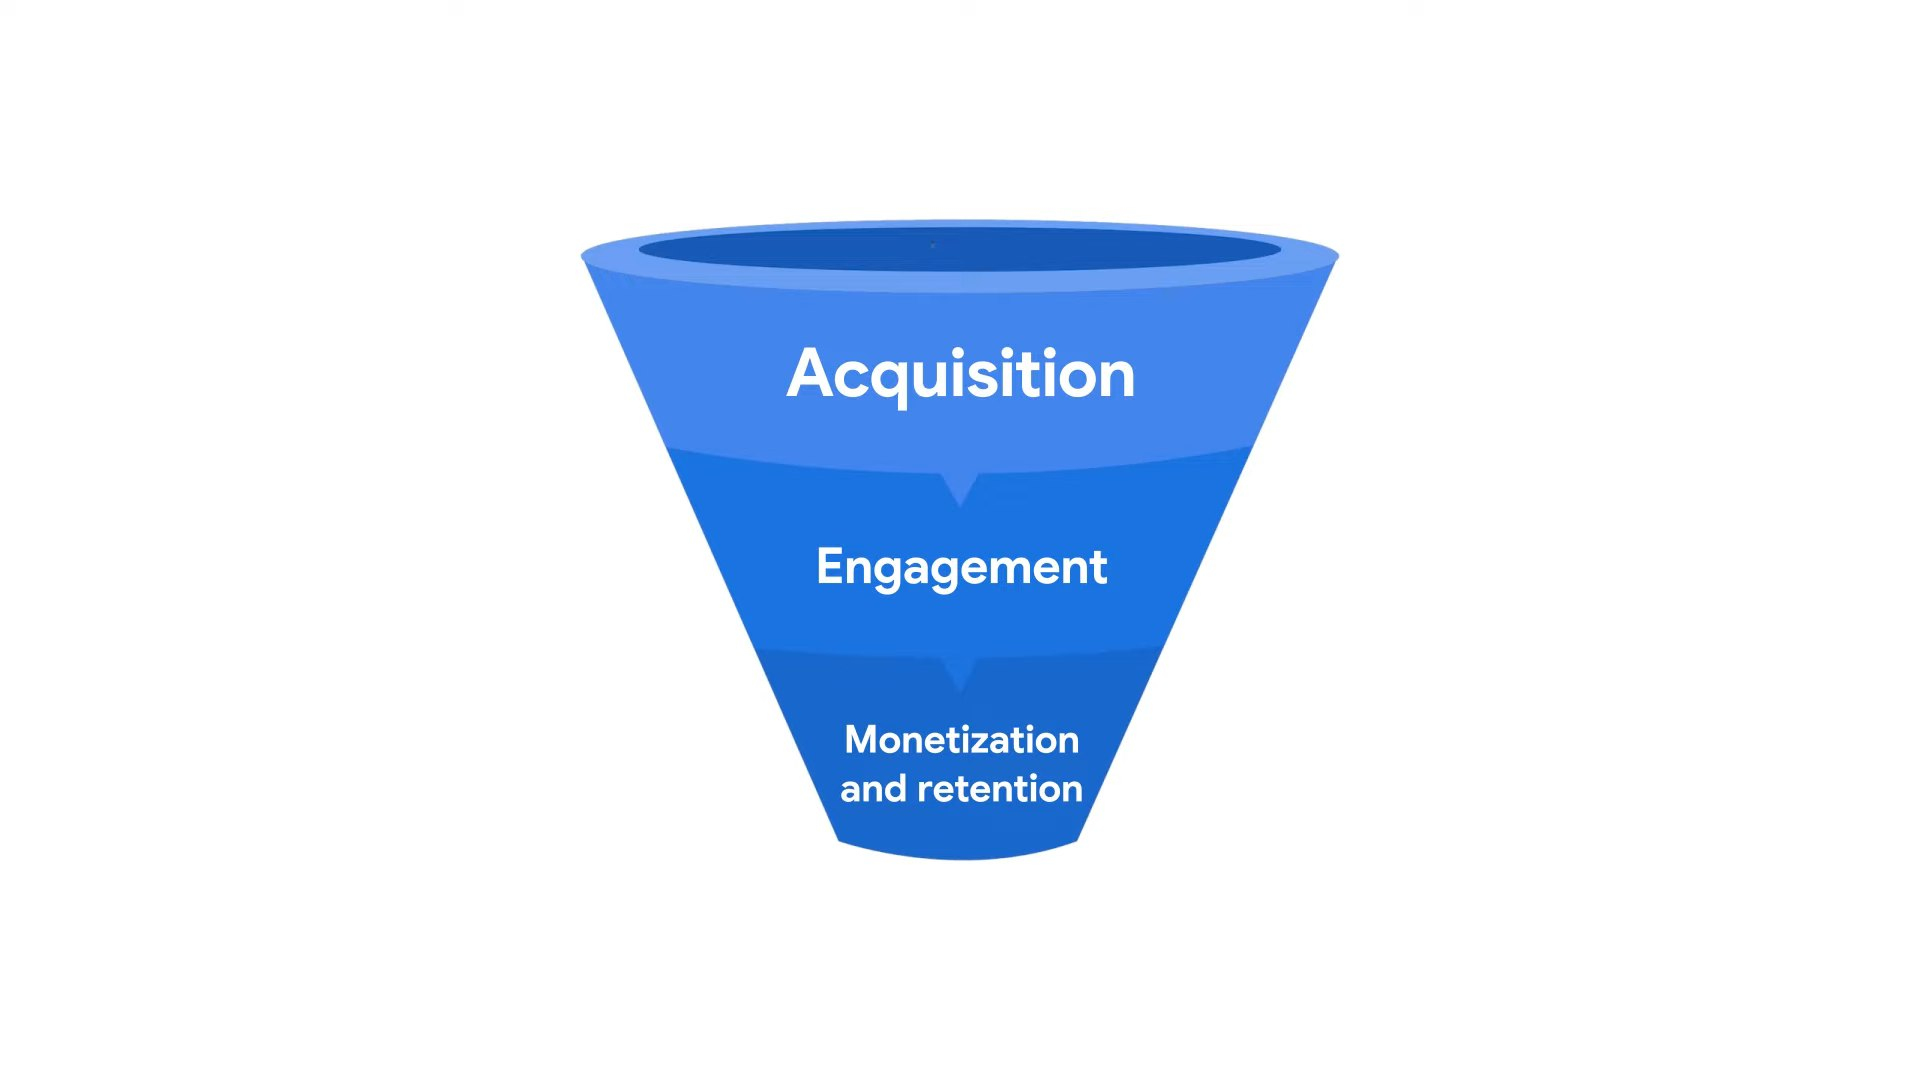
\includegraphics[width=1.0\textwidth]{obrazky-figures/funnel.jpg}
	\caption{Marketingový trychtýř. Vzato z videa: \href{https://www.youtube.com/watch?v=3faSiEX0jSg&list=PLI5YfMzCfRtZNBRmhTEJkcHYvN_x_wpxM&index=2&ab_channel=GoogleAnalytics}{https://www.youtube.com/}}
\end{figure}

Data rozdělená do těchto kategorií pomáhají lépe pochopit, co přesně zákazníky zajímá, vytvářet na jejich základě statistiky a zlepšovat firemní politiku, aby přilákala více lidí.

Pro sledování interakce uživatelů s webem poskytuje služba Google Analytics takzvaný {\it tag} -- malý úryvek kódu, který by měl být přidán do HTML kódu každé stránky webu hned pod prvek \texttt{<head>}. Podstatou tohoto úryvku je shromažďování informací o uživatelích a jejich odesílání ve formě událostí. Například když člověk navštíví webové stránky poprvé, služba Google Analytics o tom provede záznam jako o události {\it first open event}. Stejně tak bude shromažďována, analyzována a přeformátována do podoby informací jakákoli interakce se stránkami, formuláři a dalšími částmi webu, včetně odchodů, které si pak majitel webu může prohlédnout a vyvodit na jejich základě závěry pro zlepšení svého produktu~\cite{analitic}.

Kromě analytiky se tento {\it tag} používá pro následující marketingové~\ref{sec:2:marketing} a remarketingové účely~\ref{sec:2:remarket}.
\bigskip
\subsection*{Google {\it tag}}
Po registraci do služby Google Analytics~\cite{accountA} obdrží uživatelé standardní {\it tag} pro sledování:
\bigskip
\bigskip
\bigskip
\bigskip
\bigskip
\bigskip
\bigskip
\begin{lstlisting}[caption=Google Tag Script, label=google-tag-script]
<!-- Google tag (gtag.js) -->
<script async src="https://www.googletagmanager.com/gtag/js?id=XXXXX"></script>
<script>
  window.dataLayer = window.dataLayer || [];
  function gtag(){dataLayer.push(arguments);}
  gtag('js', new Date());

  gtag('config', 'XXXXX');
</script>
\end{lstlisting}

Pro správné fungování běžného sledování stačí na stránku přidat pouze jeden tento {\it tag}. Další {\it tagy} nejsou potřeba. Neznamená to však, že by se tento {\it tag} omezoval na práci s jednou službou Google. Pomocí příkazu \texttt{config} k {\it tagu} je možné připojit více produktů Google pomocí identifikátorů jednotlivých služb, které jsou generovány samotným účtem~\cite{gtag}.

První část skriptu je zodpovědná za asynchronní načítání souboru \texttt{gtag.js}, který je potřebný pro spuštění sledování a sběru informací ze stránky~\cite{gtag}.

\begin{enumerate}
  \item{Poté se vytvoří nebo aktualizuje objekt \texttt{dataLayer}, který bude sloužit k přenosu informací do účtu~\cite{dataLayer}.}
  \item{Funkce \texttt{gtag()\{dataLayer.push(arguments);\}} -- tato funkce přidává do objektu \texttt{dataLayer} události, jako jsou kliknutí, návštěvy stránek, dokončení formuláře atd~\cite{dataLayer}.}
  \item{\texttt{gtag('js', new Date())} -- tento řádek inicializuje funkci \texttt{gtag} s časovým razítkem~\cite{gtag}.}
  \item{\texttt{gtag('config', 'XXXXX')} -- poslední řádek udává ID uživatele, kterému mají být výsledky odeslány, a zahajuje sběr dat~\cite{idGoogle}.}
\end{enumerate}

V této části se podrobněji zaměřím na technologii \texttt{GTag}, její připojení, specifiku použití a funkčnost, kterou poskytuje. Především je třeba poznamenat, že \texttt{GTag} není určen pro integraci do mobilních aplikací. Jeho použití je omezeno na webové prostředí -- používá se pouze pro webové stránky produktů nebo služeb, což zcela odpovídá tématu mého studia v rámci této práce. \texttt{GTag} má funkční ekvivalent -- \texttt{GTM} (Google Tag Manager), se kterým se vzájemně vylučuje. V případech, kdy společnost používá účet \texttt{GTM} pro implementaci analytiky, sběr dat a integraci s jinými službami Google, potřeba \texttt{GTag} odpadá. Důvodem je to, že Google Tag Manager ve skutečnosti plní všechny stejné funkce, které poskytuje \texttt{GTag}, ale dělá to flexibilnějším a škálovatelnějším způsobem. \texttt{GTM} je obzvláště užitečný pro produkty, které jsou v procesu aktivního vývoje nebo častých změn, protože umožňuje upravovat logiku sledování bez nutnosti přímo měnit kód webu~\cite{gtag}.

Tato část se soustředí konkrétně na \texttt{GTag} jako samostatný skript zobrazený ve výpisu~\ref{google-tag-script}, který se vkládá přímo do HTML kódu stránky. \texttt{GTag} nebo \texttt{gtag.js} je nástupcem Universal Analytics (UA), který používal skript \texttt{analytics.js}, a ještě dříve klasické \texttt{ga.js} a \texttt{urchin.js}. \texttt{GTag} je tedy moderní evolucí analytiky, která spojuje několik nástrojů do jednoho skriptu a výrazně zjednodušuje implementaci na straně klienta~\cite{gtag}.

Kromě toho bych chtěla popsat další funkce, které \texttt{GTag} umožňuje používat na webové stránce. Je třeba poznamenat, že aby \texttt{GTag} fungoval správně, je nutné vložit fragment skriptu do sekce \texttt{<head>} HTML dokumentu. Po načtení skriptu \texttt{GTag} na straně klienta okamžitě začne provádět základní funkce: inicializaci účtu, přenos standardních parametrů prohlížení stránky a připravenost ke zpracování dalších událostí~\cite{idGoogle}.

\bigskip
\texttt{GTag} poskytuje řadu funkcí pro interakci s analytickými a reklamními službami Google. Mezi klíčové funkce patří registrace událostí (\texttt{events}), nastavení globálních parametrů pomocí příkazu \texttt{set} a nastavení konfigurací pomocí příkazu \texttt{config}~\cite{idGoogle}. 

\bigskip
Příkaz \texttt{event}: sleduje události, umožňuje odesílat shromážděné údaje o interakci uživatele se stránkou do připojeného produktu Google, který je určen v příkazu \texttt{config}. Má následující podobu~\cite{idGoogle}:
\begin{lstlisting}[caption=Event command]
gtag('event', 'event_name', {
  'key': 'value',
});
\end{lstlisting}

Existují dva základní typy událostí, které lze pomocí tohoto příkazu zaregistrovat:
\begin{itemize}
    \item Doporučené události(\textbf{Recommended events}) jsou předem definované události, které mají pevné páry klíčů a formát hodnot~\cite{idGoogle}. Příklady názvů standardizovaných událostí jsou: \texttt{purchase} -- zaznamenává skutečnost, že uživatel zakoupil zboží; \texttt{login} -- označuje přihlášení uživatele do účtu. A mnoho dalších událostí, které je možné najít v seznamu~\cite{listEvent}.
    \item Uživatelské události(\textbf{Custom events}) jsou události definované vývojářem samostatně podle logiky jeho webu. Lze vytvářet vlastní názvy událostí a jejich struktury ve formátu klíč-hodnota. To umožňuje zaznamenávat specifické interakce, které nejsou pokryty doporučenými událostmi.
\end{itemize}
 Každá událost musí být přiřazena ke konkrétnímu prvku na stránce, například tlačítku nebo odkazu. Když uživatel s tímto prvkem interaguje, událost se aktivuje a data se odešlou do zdroje spojeného s {\it tagem}. Shromážděné informace lze použít nejen pro analýzu chování uživatelů, ale také pro marketingové a remarketingové účely~\cite{idGoogle}.

\bigskip
Příkaz \texttt{set} nastavuje globální parametry, které budou automaticky použity na všechny následující události na stránce. Syntaxe vypadá následovně~\cite{idGoogle}:
\begin{lstlisting}[caption=Set command]
gtag('set', 'parameterName');

gtag('set', {'currency': 'EUR'});
\end{lstlisting}
V uvedeném příkladu je nastavena měna \texttt{"EUR"} jako základní pro zpracování událostí souvisejících s cenami nebo příjmy. Kromě toho existují speciální kontrolní parametry, které mohou být spojeny jak s konfiguracemi práce {\it tagu}, tak s událostmi. Příkladem může být parametr \texttt{send\_to}, který určuje, na který zdroj nebo účet budou odeslány informace~\cite{controlParam}

V závěru je uvedený kód~\ref{google-tag-script} základním příkladem nastavení \texttt{gtag.js} -- standardního sledovacího {\it tagu} od Google. Ten slouží jako základ pro integraci různých nástrojů Google, jako jsou Google Analytics, Google Ads a další produkty. Proto je tento {\it tag} aktivně využíván jak pro analýzu chování uživatelů, tak pro realizaci marketingových a remarketingových strategií.

\bigskip
\bigskip
Abych podrobněji prostudovala, jak skript~\ref{google-tag-script} běží a přenáší data, přidala jsem ho na svou webovou stránku do kódu HTML přímo pod element \texttt{<head>}. A pomocí vývojářského nástroje v prohlížeči jsem zkontrolovala, které požadavky jsou spojené s prací tohoto skriptu a kam byly odeslány během nejjednodušší akce -- přechodu na stránku. ID ve skriptu, který jsem přidala na svou webovou stránku, je spojeno s účtem vytvořeným v Google Analytics, takže shromážděná data jsou odesílána na server Google Analytics. 

\begin{figure}[H]
	\centering
	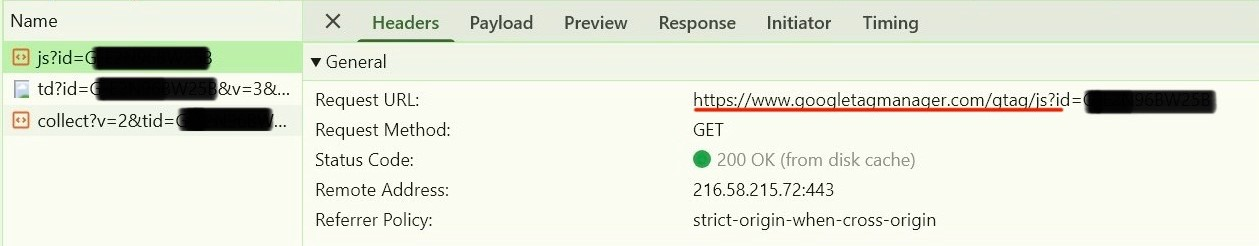
\includegraphics[width=1.0\textwidth]{obrazky-figures/req1.JPG}
	\caption{První požadavek na servery skriptů}
  \label{img:firstReq}
\end{figure}

První požadavek na Google Tag Manager stáhne samotný \texttt{gtag.js} skript do prohlížeče klienta.

\begin{figure}[H]
	\centering
	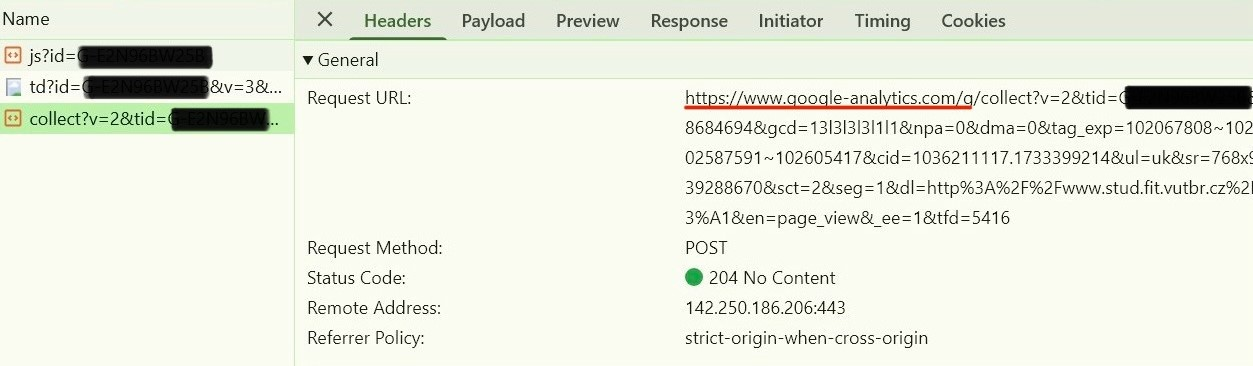
\includegraphics[width=1.0\textwidth]{obrazky-figures/req2.JPG}
	\caption{Druhý požadavek na servery skriptů}
  \label{img:secondReq}
\end{figure}

Poslední požadavek skriptu je odeslán na server Google Analytics, který přímo předá údaje shromážděné skriptem o uživateli a události, která se stala. V tomto případě se jedná o zobrazení stránky, což lze ověřit pohledem na hodnotu parametru \texttt{"en"} v názvu adresy URL požadavku. Tento parametr má hodnotu \texttt{page\_view}.


\section{Remarketingové skripty}
\label{sec:2:remarket}
Hlavním cílem remarketingu je přivést zpět uživatele, kteří již web navštívili, ale nedokončili pro společnost požadovanou akci. Například přidali produkt do košíku, ale objednávku neuskutečnili a z nějakého důvodu web opustili. Existuje několik typů remarketingu: cookie-based audiences a custom audiences. Obě metody rozdělují návštěvníky do cílové skupiny -- skupin lidí vytvořených na základě jejich akcí ve vztahu k webu nebo reklamě. 

\subsection*{Cookie-based audiences}
Remarketing založený na cookie-based audiences používá cookie nebo sledovací zařízení v prohlížeči uživatele, které ukládá informace o tom, do které kategorie cílové skupiny uživatel patří. Tyto informace pomáhají reklamní síti vybírat reklamy, které se budou zobrazovat na dalších webových stránkách, které daná osoba navštíví.

\subsection*{Custom audiences}
Custom audiences využívá informace o uživatelských datech, jako je e-mail, telefonní číslo nebo ID zařízení, z něhož návštěvník přichází, k zařazení do požadované cílové skupiny. Společnost Google následně ověří, zda uživatel patří do určité cílové skupiny, například na základě jeho e-mailové adresy~\cite{googleAds}. 

\subsection*{Nastavování cílových skupin}
Vytvoření publika pro remarketing se nastavuje v několika krocích. Nejprve je třeba vytvořit novou cílovou skupinu lidí v účtu Google Ads a vybrat {\it tag}, který přidá návštěvníka do této cílové skupiny během konkrétní události.  A poté ten {\it tag} přidat na potřebné stránky webu. Hlavní {\it tag} pro remarketing vypadá stejně jako pro analytiku, protože bude nejen shromažďovat informace o návštěvnících, ale také přenášet data do požadovaného účtu Google Ads. Po nastavení fragmentu kódu můžete ve svém účtu vytvářet a spravovat cílové skupiny. Cílovou skupinu lze vytvořit jak na základě navštívených stránek, tak na základě akcí, jako je vyplnění formulářů, objednání zboží atd.

Dynamický remarketing je název pro remarketing, který umožňuje společnostem nejen zobrazovat hlavní reklamy, ale také je přizpůsobit každému zákazníkovi a přivést ho zpět na web, aby dokončil to, co na něm začal~\cite{dynRemarket}.

Pro nastavení cílové skupiny je v Google Ads k dispozici sekce Audience manager, která poskytuje potřebné {\it tagy} pro požadavky společnosti a možnost správy cílové skupiny. 

\subsection*{Aukce}
O tom, jaká reklama se zobrazi na stránkách navstívených uzivatelem, se rozhoduje v reklamnich aukcich. Společnosti, které mají inzeráty na zadaná klíčová slova nebo jejichž cílová skupina odpovídá těmto klíčovým slovům, nabízejí své inzeráty a soutěží o jejich umístění. Vítěze aukce určuje několik faktorů \cite{rtb}:
\begin{enumerate}
  \item \textbf{Bid}(nabídka). Tento faktor určuje, kolik je každá společnost ochotna zaplatit za kliknutí osoby, respektive maximální nabídku, kterou lze zaplatit.
  \item \textbf{Quality Score}(skóre kvality). Aby bylo zajištěno, že se uživatelům zobrazí pouze relevantní reklamy, hodnotí společnost Google každou možnost v aukci od 1 do 10. 
\end{enumerate}
Poté se vypočítá hlavní kritérium výběru -- Max bid $\times$ Quality Score = Ad Rank. Uživateli se zobrazí reklama s nejvyšší hodnotou Ad Rank~\cite{auction}.


\section{Marketingové skripty}
\label{sec:2:marketing}
Po vytvoření a nastavení účtu Google Ads začne kampaň okamžitě fungovat, což znamená, že se vytvořené reklamy budou účastnit aukcí a zobrazovat se uživatelům. Do kódu svých webových stránek nemusíte integrovat nic dalšího. Pro zlepšení výkonu společnosti, včasnou reakci na změny zájmu publika, přilákání pozornosti nových návštěvníků a podobně se však vytvářejí marketingové skripty, které se integrují do účtu Google Ads. Podrobněji je a jejich účel popíšu v této sekci.

Marketingové skripty slouží k automatizaci a optimalizaci marketingových procesů v účtu Google Ads. Tyto skripty jsou kódy napsané v jazyce JavaScript, které mohou pomoci se změnou nabídek, pozastavením reklamních skupin, přidáním klíčových slov atd. Na základě shromážděných informací nebo nastavených podmínek mohou tyto úryvky kódu měnit různé aspekty kampaně, aby se zlepšil výkon reklamy a přilákalo se větší cílové skupiny návštěvníků.

Tyto skripty je třeba přidat a nakonfigurovat přímo v účtu Google Ads. Zde je několik možností jejich použití~\cite{adsHelp}:
\begin{enumerate}
  \item Použijte externí data, například shromážděná pro analýzu Google, k inicializaci změn v reklamní kampani.
  \item Automaticky měnit prvky účtu Google Ads, například klíčová slova, reklamní skupiny, nabídky atd. Můžete je měnit jak systematicky za zvláštních podmínek, tak jednorázově, aby se shodovaly s nějakou událostí.
  \item Vytváření přehledů o průběhu marketingových kampaní.
\end{enumerate}

Skripty lze vytvářet samostatně s ohledem na potřeby inzerenta nebo lze použít hotové šablony~\cite{adsScripts} a fragmenty kódu~\cite{fragment}. 





\chapter{Blokátory založené na blokovaných URL} 
\label{ch:3}

V dnešní době nemusí být surfování na internetu tak bezpečné, jak se na první pohled zdá. Někdy se za reklamou, kterou se nám společnosti tak usilovně snaží propagovat, skrývá víc než jen zajímavá webová stránka nebo článek. Za internetovými stránkami mohou číhat podvody, phishing, nevhodný obsah a další nebezpečí. Přestože existují zákony chránící práva uživatelů internetu, například GDPR (o kterém jsem se zmínila v kapitole~\ref{ch:1}), mnohé reklamy mohou být pro návštěvníka stále škodlivé. Proto je důležité chránit své online prostředí pomocí tzv. blokátorů.

V této části se zaměřím na blokátory webového obsahu založené na seznamech blokovaných adres URL.

\section{Potenciální rizika pro uživatele na internetu}
Nejprve se však podívejme na možná rizika, kterým se lidé vystavují na internetu.

Začnu těmi nejméně nebezpečnými problémy. Inzerenti používají křiklavé titulky a obrázky, tzv. šokující obsah, aby uživatele zaujali svými reklamami. Bohužel část tohoto obsahu je z kategorie "pro dospělé", jako jsou erotické obrázky, obrázky mrzačení apod. To znamená, že obsah není určen ke sledování lidem jakéhokoli věku. Kromě nepříjemných pocitů, které při prohlížení takových reklam vznikají, mohou obsahovat kód, který uživatele ohrožuje.
Dalším problémem je bránění volnému prohlížení webového obsahu. Některé webové stránky mohou obsahovat tolik reklam, že brání volnému prohlížení informací, které člověk potřebuje~\cite{adblock}.

Větší nebezpečí samozřejmě představují reklamy, které obsahují škodlivý kód, například viry, trojské koně nebo jiné typy malwaru, které mohou infikovat počítač nebo zařízení uživatele. Interakce s podvodnými stránkami -- reklamy mohou uživatele nasměrovat na imitaci internetového obchodu nebo platebního systému. Takové stránky slouží ke krádeži důvěrných informací, jako jsou hesla nebo čísla bankovní karty~\cite{adblock}. Bohužel blokátory reklam nemohou zabránit doručení škodlivého softwaru, který již byl spuštěn. Mohou však přidat domény známých stránek, které šíří například viry, do seznamu a filtrovat požadavky na ně.

Dalším rizikem je zneužití shromažďování osobních údajů webovou stránkou nebo webovou aplikací. Platformy, jako je Instagram, TikTok, GitHub, YouTube a další, umožňují registraci pomocí stávajícího účtu na jiné sociální síti nebo službě. Tím získá webová aplikace nebo webová stránka přístup k osobním údajům uživatele uvedeným v jeho účtu a může je využít k cílení reklamy. Pokud služba není dostatečně zabezpečená, může to vést i k úniku dat. Abyste se takovému riziku vyhnuli, doporučují pečlivě číst, jaká oprávnění udělujete, a pokud možno se neregistrovat u služeb třetích stran na webových stránkách, kterým nedůvěřujete.

Při používání prohlížeče se člověk může vystavit riziku také sám. Například prohlížeč Google umožňuje ukládat registrační údaje z různých webových stránek. Přihlašovací jména, hesla  a dokonce i údaje o bankovní kartě -- aby si je člověk nemusel pamatovat a pokaždé je zadávat znovu, nabízí společnost Google uložení těchto údajů do účtu člověka a jejich automatické doplnění, když se objeví požadovaný formulář. Toho podvodníci využívají, když na webové stránky umístí skrytý formulář. Takový formulář může být skrytý na kterékoli stránce webu. Google jej automaticky vyplní uloženými údaji, které pak obdrží třetí strana. Tyto akce nejen porušují soukromí, ale mohou být také využity k podvodům. Pokud používáte Google k automatickému ukládání dat, měli byste být opatrní a používat rozšíření, která blokují skripty třetích stran. 

Aby se předešlo těmto nebezpečím a nepříjemnostem, byly vytvořeny blokátory reklam.


\section{Princip fungování blokátoru reklamy}
Princip činnosti lze popsat takto:
\begin{itemize}
  \item{ Blokátory používají filtrovací seznam a spoléhají se na pravidla filtrování, aby věděly, co mají blokovat a skrývat před uživatelem. Seznamy a pravidla popíšu podrobněji v sekci~\ref{seznam}.}
  \item{Proces filtrování probíhá, když prohlížeč odešle požadavek HTTP na server webu. Při procházení seznamu blokátor porovnává adresu URL požadavku s filtry v seznamu. Pokud je nalezena shoda, je svazek identifikován jako nežádoucí obsah a zablokován. Obvykle je blokován svazek serverů třetích stran, nikoliv ten hlavní. Například člověk navštíví zpravodajský web, kde jsou reklamy, trackery nebo analytické skripty načteny z jiného serveru, než je server zpravodajského webu. Pokud je některý z těchto prvků blokátorem detekován jako nevhodný obsah, je požadavek na něj zablokován a ze serveru není přijata žádná odpověď.}
  \item{Kromě toho může blokátor po načtení samotného zpravodajského webu projít jeho strukturu a pomocí CSS skrýt prvek s reklamou, aniž by změnil strukturu webu jako celku. }
\end{itemize}

Tímto způsobem blokátor zajistí, že uživatel zůstane na webu bezpečně, a urychlí načítání stránky, jelikož se sníží množství stahovaného obsahu. 

Jak bylo uvedeno výše, blokátory filtrují nejen digitální reklamy, ale i URL požadavky na servery, které odpovídají jejich pravidlům. To znamená, že jsou blokovány a neaktivovány také sledovací prvky, analytické, marketingové a remarketingové skripty. Tímto způsobem uživatel omezuje nežádoucí shromažďování svých osobních údajů třetími stranami.

\section{Výhody a nevýhody používání blokátorů reklam}
V dnešní době nebude pro nikoho problém najít a nainstalovat blokátor a výběr je velmi rozmanitý. Než se rozhodnete pro instalaci a výběr konkrétní služby, stojí za to zvážit, jaké jsou výhody a nevýhody blokátorů.

\subsection*{Výhody}
\begin{itemize}
  \item{Zvyšuje rychlost načítání stránek. Odfiltrování části reklam urychluje načítání stránky, snižuje spotřebu dat a šetří elektrickou energii, například baterii zařízení. Rychlost načítání stránek je podstatnou metrikou, která výrazně ovlivňuje atraktivitu webu pro uživatele. Kromě toho je to výhoda pro uživatele s omezenými internetovými tarify~\cite{adblock}.}
  \item{Ochrana před nežádoucím obsahem. Vyčistí webové stránky od zbytečných bannerů a zlepší uživatelský zážitek. Pozornost návštěvníka se nerozptyluje na spoustu oken se zbytečnými informacemi~\cite{adblock}.}
  \item{Ochrana před potenciálním malwarem. Chrání uživatele před šířením jeho osobních údajů, stahováním programů třetích stran, podvody a dalšími~\cite{adblock}. Blokátory založené na blokovaných URL, bohužel nemohou uživatele plně ochránit před neznámými sledovacími zařízeními. Podle výzkumu provedeného v článku "Missed by Filter Lists: Detecting Unknown
Third-Party Trackers with Invisible Pixels"~\cite{pixels} jsou sledovací zařízení třetích stran přítomna na 94,51 \% domén.  A dva populární metody blokování založené na EasyList\&EasyPrivacy a Disconnect list, přehlédnou 25,22 \% a 30,34 \% neznámých sledovacích zařízení.}
\end{itemize}


\subsection*{Nevýhody}
\begin{itemize}
  \item{Ztráta základních funkcí. Existují případy, kdy je blokována důležitá část obsahu, po které web ztratí svou základní funkčnost. Nesprávné zobrazení prvků a neúplná funkčnost způsobí, že web pro návštěvníky ztratí smysl~\cite{adblock}. }
  \item{Ohrožení soukromí a bezpečnosti uživatelů. Některé blokátory reklam již mohou obsahovat malware nebo shromažďovat osobní údaje uživatelů. Také některé nebezpečné reklamy nemusí být zařazeny do seznamů v případech, kdy majitelé reklam platí za to, aby nebyly blokovány. Abyste tomu předešli, měli byste si nainstalovat pouze důvěryhodné blokátory reklam~\cite{adblock}.}
  \item{Technické problémy. Webové stránky se mohou pokusit blokování obejít, což povede k technickým problémům na počítači uživatele~\cite{adblock}.}
\end{itemize}

\section{Rozšíření pro prohlížeč, která blokují webový obsah}
V této části se budu více věnovat rozšířením prohlížeče. Jako příklad uvedu tři z nejrozšířenějších a nejznámějších rozšíření určených k blokování reklam v prohlížečích. Tyto nástroje fungují na základě seznamů blokovaných URL adres, které automaticky filtrují nežádoucí obsah při načítání stránky. Mezi nimi bude uBlock Origin, Adblock Plus a Ghostery. Každý z nich má své unikátní výhody a silné stránky, díky kterým vynikají mezi ostatními existujícími rozšířeními pro blokování. Podle výsledků testování, které provedl tým PC MAG a zveřejnila jejich Senior Security Analyst Kim Key, Adblock Plus byl uznán jako nejlepší pro povolení reklam -- díky flexibilnějšímu systému výjimek a podpoře přípustných reklam. uBlock Origin byl uznán jako nejlepší řešení z hlediska customizace -- možnost podrobně nastavit blokování. Ghostery zase získal vysoké hodnocení za uživatelské rozhraní, které je jednoduché a intuitivní~\cite{pcmag}.

Nyní přejdu k podrobnějšímu popisu každého z uvedených rozšíření, začnu s uBlock Origin.

\subsection*{uBlock Origin Lite}
Bohužel po nasazení nové verze platformy rozšíření Manifest 3 v prohlížeči Google Chrome bylo na oficiálních stránkách uBlock Origin oznámeno, že v důsledku změn platformy dochází k závažným technickým potížím~\cite{ublock}. Z tohoto důvodu již není plná verze rozšíření uBlock Origin ve své klasické podobě v prohlížeči Google Chrome podporována. Pro uživatele, kteří chtějí pokračovat v používání Chromu, však vývojáři vydali alternativu -- verzi s názvem uBlock Origin Lite. Tento analog je přizpůsoben nové verzi platformy rozšíření a ačkoli zachovává část základních funkcí, je třeba si uvědomit, že se nejedná o plnohodnotnou náhradu klasického uBlock Origin~\cite{pcmag}. Pro ty, kteří chtějí pokračovat v používání plné verze rozšíření, je doporučeno přejít na jiné prohlížeče, které nepřecházejí na Manifest 3, jako je například Firefox~\cite{ublock}. 

\begin{figure}[H]
	\centering
	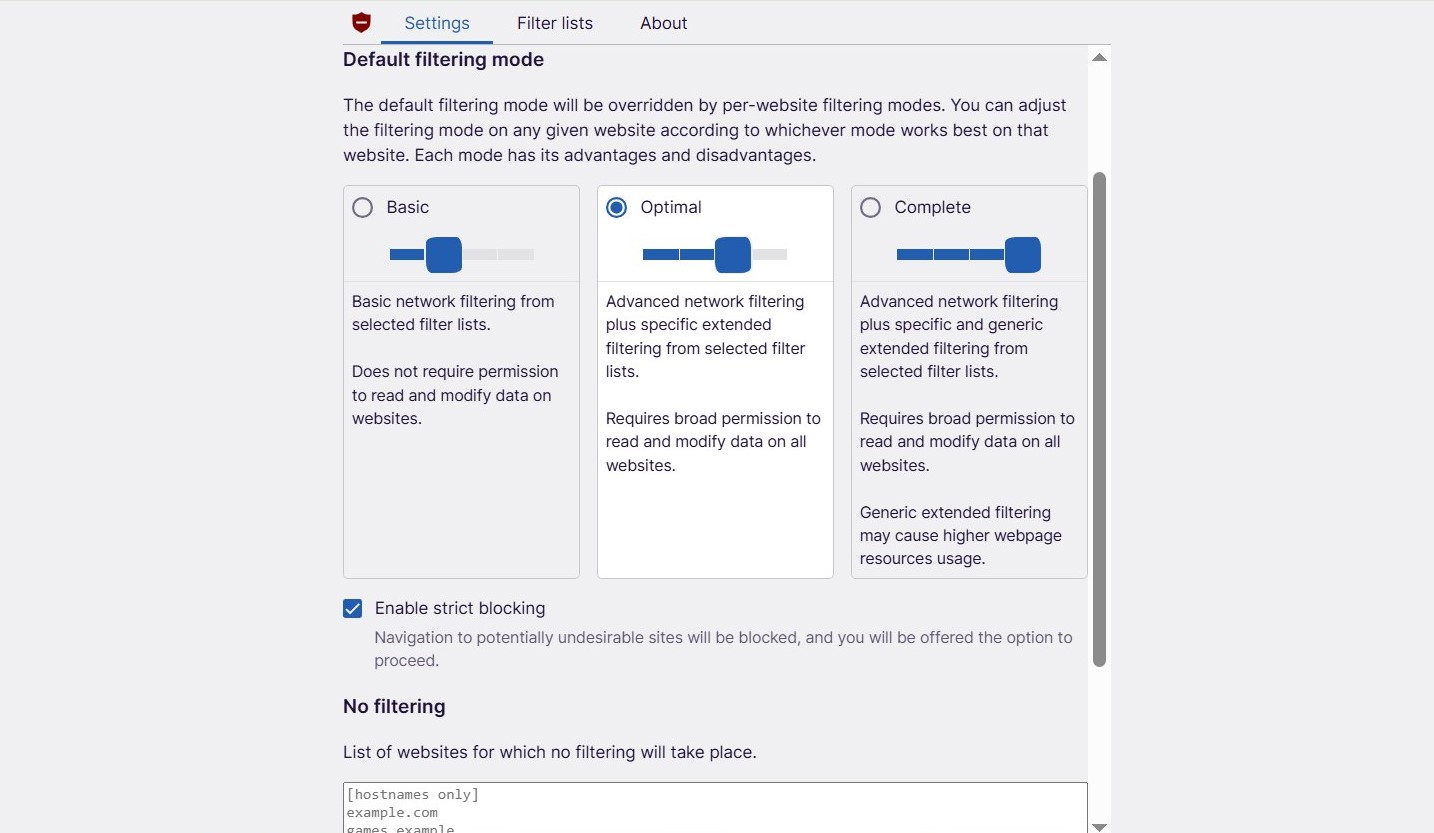
\includegraphics[width=0.9\textwidth]{obrazky-figures/uBlockLite.jpg}
	\caption{Snímek obrazovky s nastavenim rozšíření uBlock Origin Lite, které jsem si stáhla}
        \label{img:uBlock}
\end{figure}

Navzdory zjednodušení má uživatel v lite verzi stále k dispozici základní nástroje pro flexibilní  nastavení blokování, jako je výběr seznamů blokování, vizuální správa povolených nebo blokovaných prvků na stránce a další. To umožňuje lépe přizpůsobit chování blokátoru vlastním potřebám. Jednou z klíčových vlastností uBlock Origin Lite je přítomnost několika režimů blokování, které lze měnit přímo přes rozhraní rozšíření. Uživatel si může vybrat jednu ze tří úrovní kontroly: základní, optimální nebo úplný režim. Každý z těchto režimů odpovídá určité úrovni intenzity filtrování požadavků odesílaných prohlížečem na externí servery.

Čím vyšší je zvolený režim, tím více filtračních pravidel a blokovacích seznamů se použije, čímž se odpovídajícím způsobem zvyšuje počet blokovaných prvků na webové stránce, jako jsou trackery, analytické skripty, reklamní zdroje a další podobné objekty. Například základní režim zajišťuje nejnižší úroveň zásahu. Optimální režim je považován za ideální kompromis -- zajišťuje účinnou ochranu bez nadměrné spotřeby zdrojů nebo problémů se zobrazením webu. Plný režim zase předpokládá nejagresivnější filtrování, ale může vyžadovat další oprávnění v prohlížeči, například přístup k obsahu stránek nebo změnu jejich prvků. Z tohoto důvodu může tento režim vést ke zvýšení zatížení stránky. 

Kromě automatické filtrace nabízí rozšíření také možnost ručního řízení výjimek. Uživatel může zejména přidávat jednotlivé domény do tzv. bílého seznamu, který je zobrazen ve spodní části snimku obrazovky~\ref{img:uBlock}. To znamená, že všechny požadavky související s těmito weby nebudou blokovány bez ohledu na zvolený režim. Tento přístup je vhodný v případech, kdy je pro uživatele důležité zachovat plnou funkčnost určitého zdroje nebo když blokování brání v práci služby, kterou uživatel potřebuje.

V nastavení rozšíření je také možné ručně vybrat, které seznamy pravidel se budou používat. Například uživatel může zapnout nebo vypnout používání EasyList, EasyPrivacy a dalších. To poskytuje větší flexibilitu a umožňuje nastavit chování blokovače co nejpřesněji -- podle individuálních požadavků uživatele nebo testovacího prostředí, ve kterém je toto rozšíření používáno. 

\subsection*{Adblock Plus}
Další rozšíření, které podrobně rozeberu ve své práci, je Adblock Plus. Název tohoto nástroje je starý a v oblasti blokování reklam dobře známý~\cite{pcmag}. Jedním z hlavních rozdílů Adblock Plus oproti dvěma ostatním zmíněným rozšířením je existence bezplatné i placené verze.

\begin{figure}[H]
	\centering
	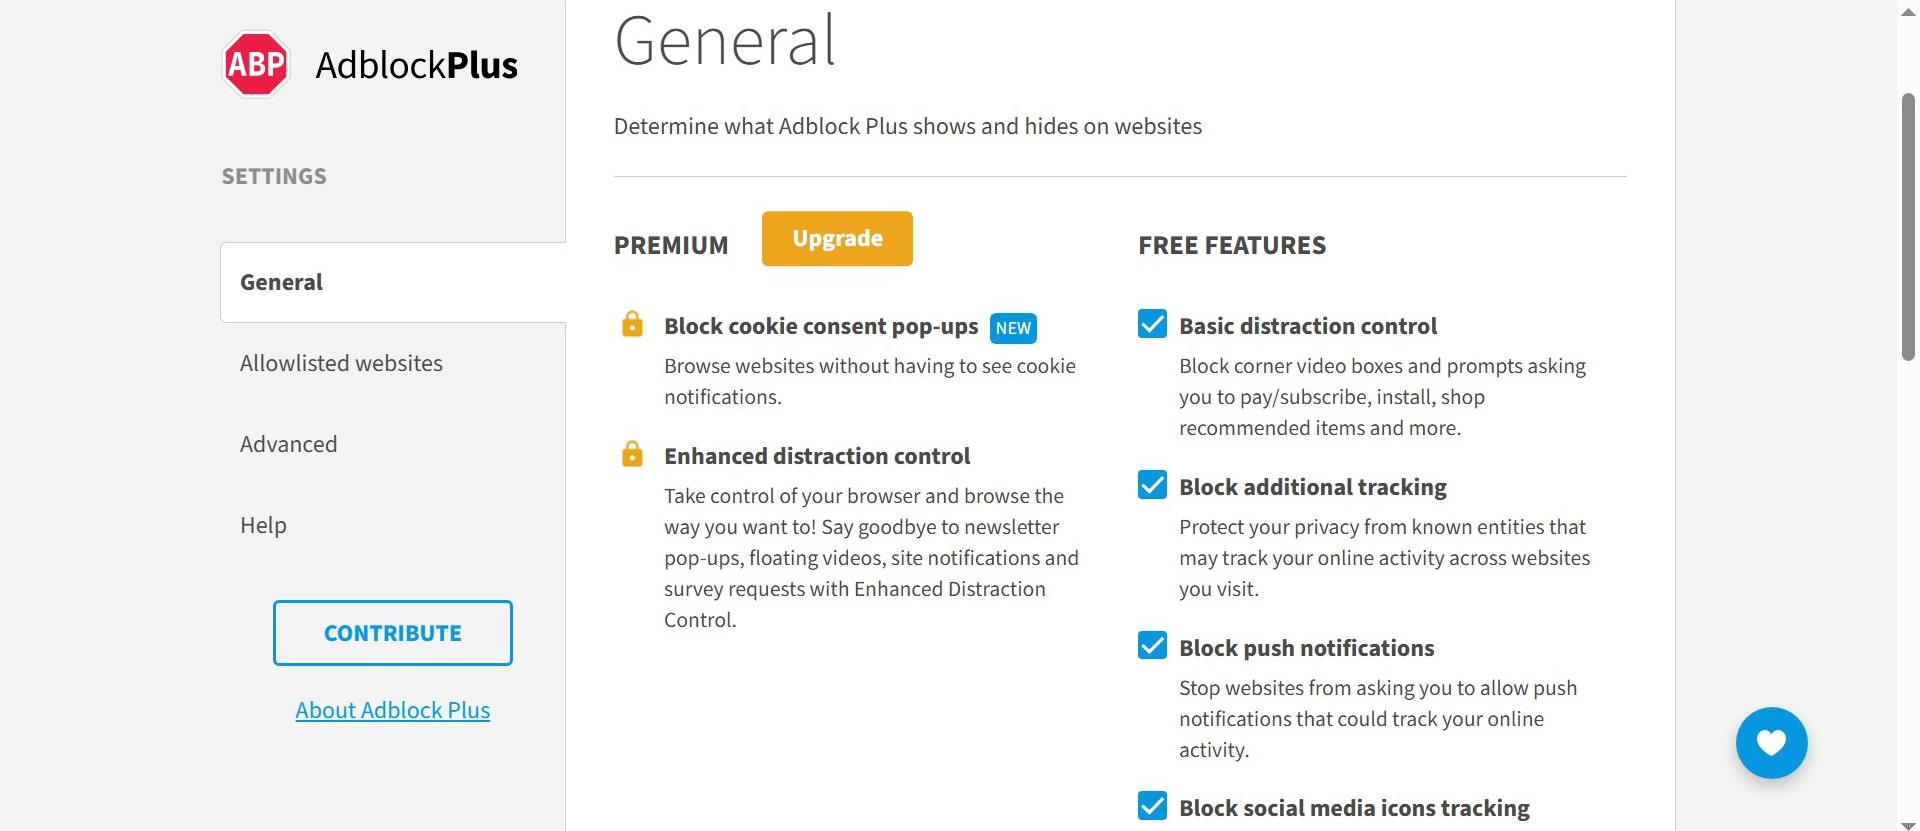
\includegraphics[width=1.0\textwidth]{obrazky-figures/AdBlockPlus2.jpg}
	\caption{Snímek obrazovky s nastavenim rozšíření Adblock Plus, které jsem si stáhla}
        \label{img:AdBlock1}
\end{figure}

Jak je mozné vidět na snímku obrazovky~\ref{img:AdBlock1}, placená verze nabízí další možnosti, které mohou být užitečné pro uživatele, kteří chtějí zvýšit svůj komfort při prohlížení stránek a úroveň ochrany soukromí. Mezi další možnosti patří automatické blokování vyskakovacích oken, které vyžadují souhlas s používáním souborů cookie. Placená verze tak vytváří čistší prostor pro uživatele při jeho přebývání na internetu.

\begin{figure}[H]
	\centering
	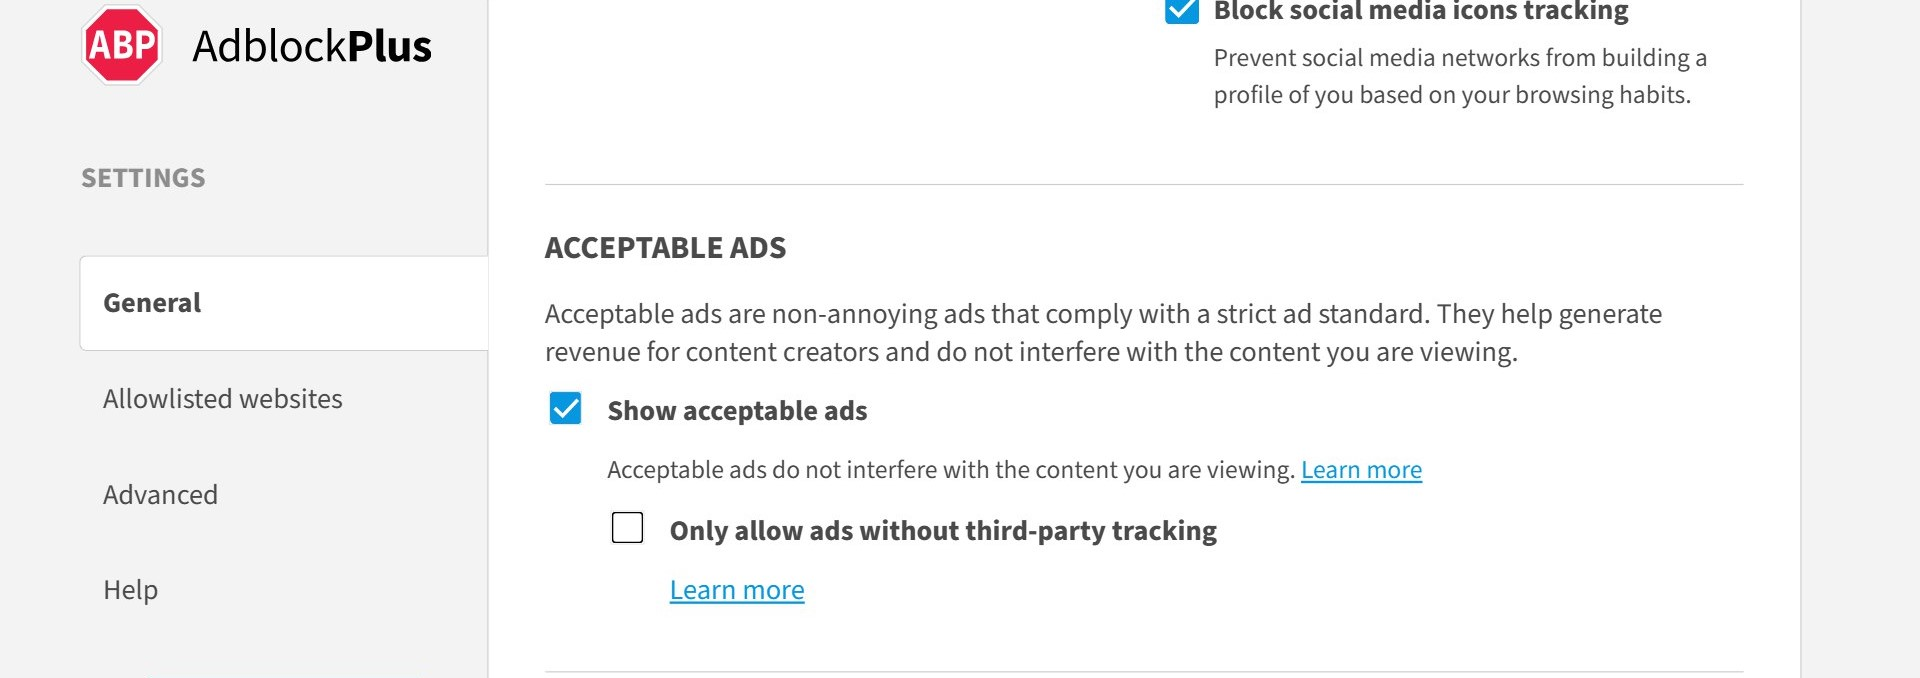
\includegraphics[width=1.0\textwidth]{obrazky-figures/AdBlockPlus3.jpg}
	\caption{Snímek obrazovky s nastavenim rozšíření Adblock Plus, které jsem si stáhla}
        \label{img:AdBlock2}
\end{figure}

Další vlastností Adblock Plus je možnost blokovat ne všechny reklamy na stránkách. Tuto možnost lze ručně zapnout a vypnout v nastavení rozšíření, které je zobrazeno na snímku obrazovky~\ref{img:AdBlock2}. Pokud je parametr "Povolená reklama" aktivován, Adblock Plus bude propouštět reklamní bloky, které považuje za nerušivé, a ty se budou zobrazovat na stránce prohlížeče uživatele. 
\begin{figure}[H]
	\centering
	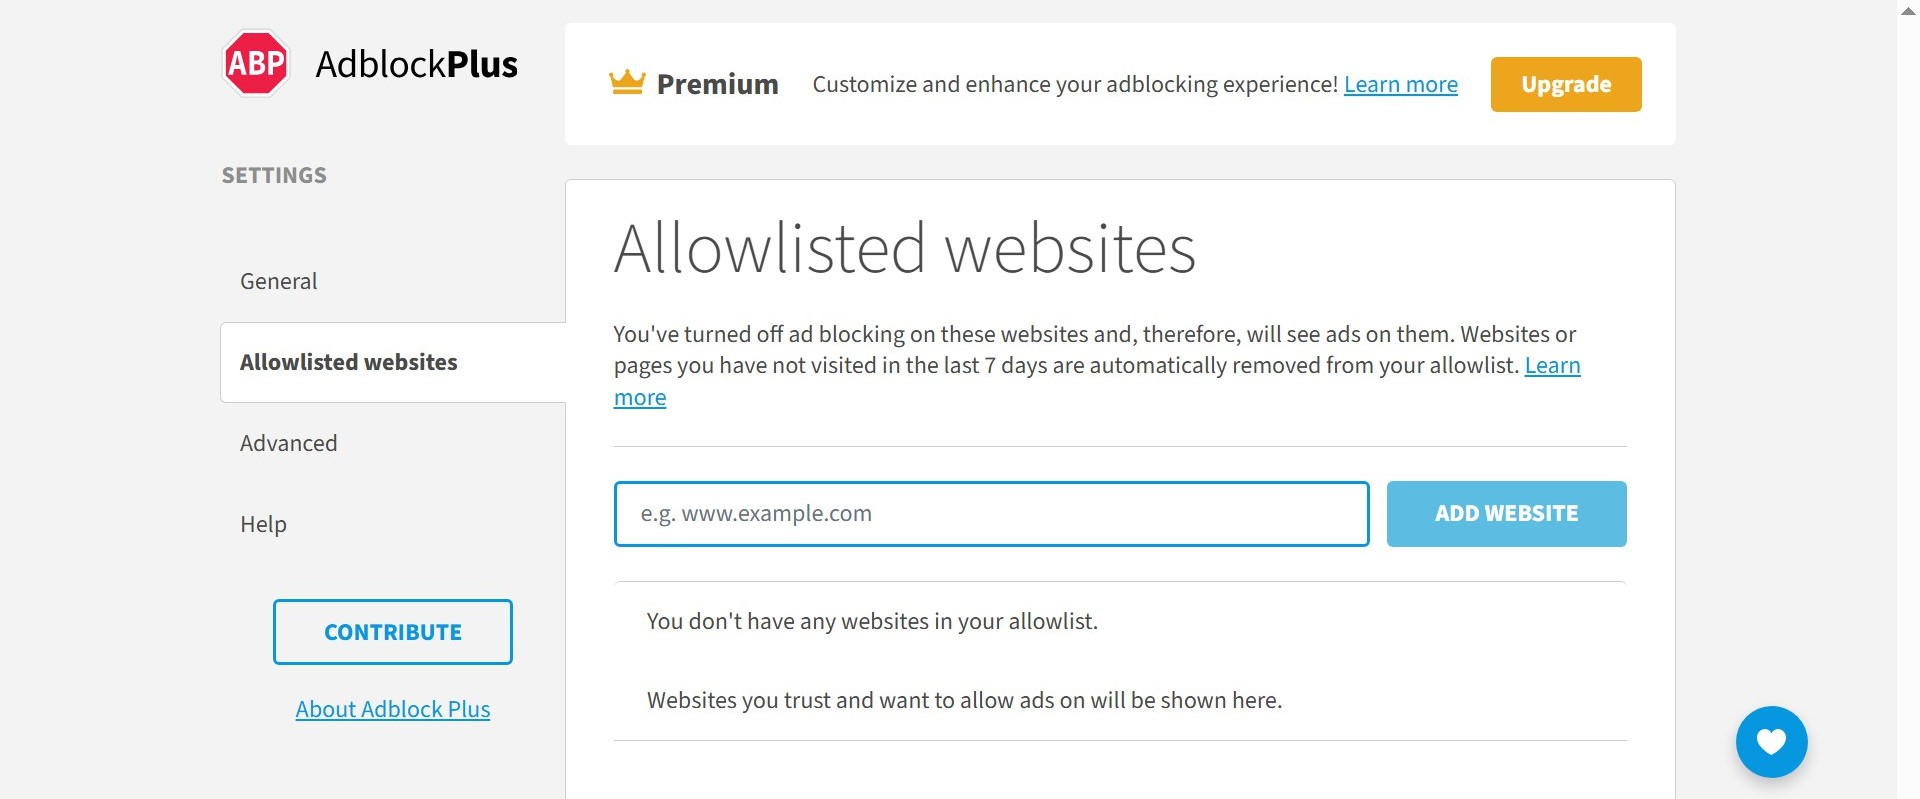
\includegraphics[width=1.0\textwidth]{obrazky-figures/AdBlockPlus.jpg}
	\caption{Snímek obrazovky s nastavenim rozšíření Adblock Plus, které jsem si stáhla}
        \label{img:AdBlock3}
\end{figure}
Stejně jako v uBlock Origin Lite, v Adblock Plus je implementována funkce povolených webů -- seznam webových zdrojů, které uživatel ručně přidá do výjimek. Stránky z tohoto seznamu nejsou ovlivněny obecnými pravidly filtrování a nebudou rozšířením blokovány. Tato možnost je implementována v sekci nastavení \texttt{"Allowlisted websites"}, která je zobrazena na snímku obrazovky~\ref{img:AdBlock3}. Kromě toho může uživatel vybrat, které seznamy filtrování budou použity pro aktuální relaci prohlížení -- zapnutím a vypnutím příslušných názvů seznamů v nastavení rozšíření.

\subsection*{Ghostery}
Poslední rozšíření, které jsem zahrnula do svého přehledu, je Ghostery. Na rozdíl od uBlock Origin, Ghostery nenabízí tak vysokou úroveň přizpůsobení. To však neznamená, že je méně účinný. Ghostery se osvědčil jako spolehlivý blokátor reklam a získal nejvyšší hodnocení od testovacího webu AdBlock a EFF's Cover Your Tracks. Jednou z nejsilnějších stránek rozšíření je jeho intuitivní a uživatelsky přívětivé rozhraní~\cite{pcmag}. 
\begin{figure}[H]
	\centering
	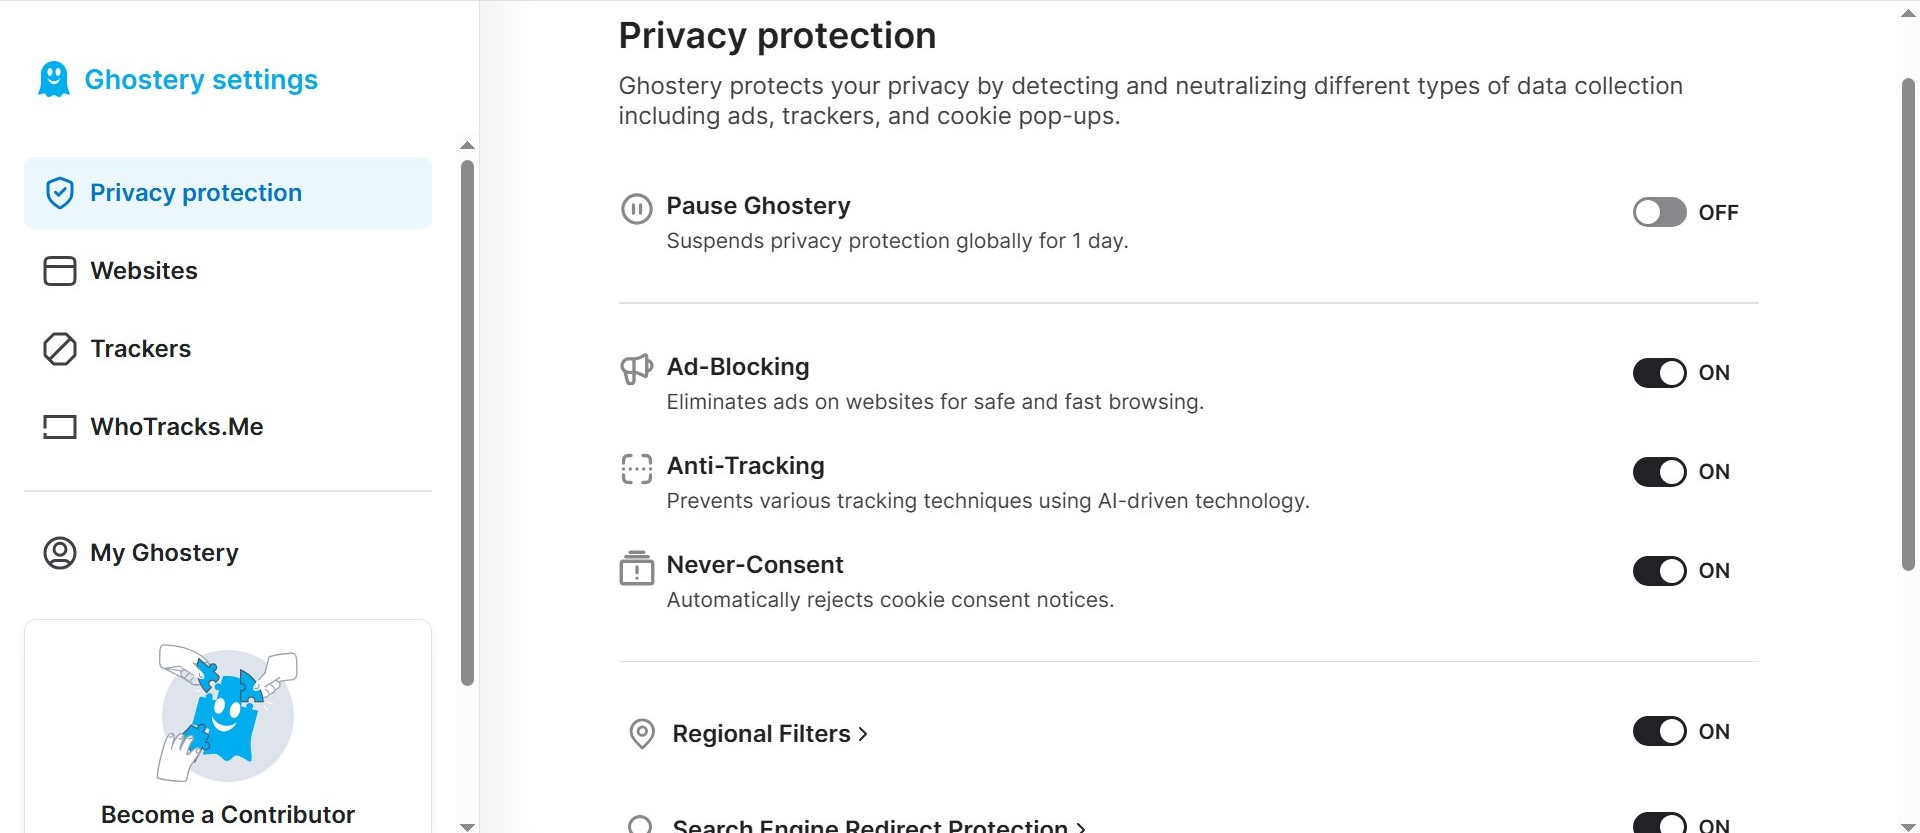
\includegraphics[width=1.0\textwidth]{obrazky-figures/Ghostery.jpg}
	\caption{Snímek obrazovky s nastavenim rozšíření Ghostery, které jsem si stáhla}
        \label{img:Ghostery}
\end{figure}
Ghostery lze použít ihned po stažení, bez nutnosti nastavovat složité doplňkové parametry. Je však třeba vzít v úvahu, že je nutné zapnout nastavení soukromí rozšíření, než bude Ghostery schopen blokovat reklamy, trackery a další nežádoucí prvky v prohlížeči uživatele. 

\subsection*{Seznamy filtrů}
\label{seznam}
Nejčastěji používaným rozšířením je \textbf{EasyList}. EasyList je hlavní seznam filtrů pro blokování reklam, byl původně vyvinut pro Adblock, ale nyní je kompatibilní s mnoha dalšími blokátory, jako jsou Adblock Plus, uBlock Origin a AdGuard. Je to také nejoblíbenější seznam, který se používá jako základ pro desítky dalších kombinovaných a doplňkových seznamů filtrů. Tento seznam je neustále aktualizován a doplňován o další filtry. Mezi přírůstky tohoto seznamu patří EasyList Cookie List a EasyPrivacy. 

\textbf{EasyList Cookie List}, jak název napovídá, blokuje bannery s cookie a další zprávy související se soukromím. 

\textbf{EasyPrivacy} je další seznam filtrů zaměřený na odstranění všech forem sledování uživatelů. Tím jsou chráněny osobní údaje návštěvníků~\cite{easylist}.

V případě potřeby může uživatel sám vytvářet nebo přidávat filtry, pokud dodrží stanovenou syntaxi pravidel filtrování~\cite{filterRule}.

Pro úplné pochopení blokovacího filtru je vhodné rozebrat základní pravidla jeho syntaxe. Zdrojem, ze kterého jsem uvedené informace převzala, byla oficiální dokumentace Adblock Plus, jejíž pravidla jsou použita ve výše popsaných seznamech EasyList, EasyPrivacy a dalších.

\begin{itemize}
    \item \texttt{||} -- objevuje na začátku řádku, znamená, že URL s uvedenou doménou bude blokována. Například tento řetězec \texttt{||example.com/} bude blokovat obě adresy \\
    \texttt{http://www.example.com/} a \texttt{http://example.com/}~\cite{filterRule}.
    \item \texttt{*} -- znamená, stejně jako v regulárních výrazech, libovolný počet libovolných znaků~\cite{filterRule}.
    \item \texttt{\^} -- znak oddělovače může znamenat konec domény, začátek parametrů apod~\cite{filterRule}.
    \item \verb||| -- znamená začátek nebo konec URL~\cite{filterRule}.
    \item \verb|$| -- označuje konkrétní typy požadavků, které by měly být blokovány. Je spojen se slovem, které označuje typ. Jako například \verb|$script|, \verb|$image|, \verb|$stylesheet| a \verb|$third-party|, které se používají nejčastěji~\cite{filterRule}.
    \item \verb|~| -- znamená inverzní použití, například \verb|~script| znamená nepoužití pravidla na adresy URL, které obsahují skript~\cite{filterRule}.
    \item \texttt{domain=example.com} -- může se objevit na konci řetězce s URL, znamená, že filtr by měl být aplikován na URL obsahující tuto domenu \texttt{example.com}~\cite{filterRule}.
    \item \texttt{@@} -- tento znak se objevuje na začátku řetězce, který je výjimkou. Například toto pravidlo \texttt{@@||example.com/} znamená, že blokátor nebude filtrovat adresy URL obsahující doménu nebo část domény \texttt{example.com/}~\cite{filterRule}.
    \item \texttt{!} -- řetězce začínající vykřičníkem jsou komentáře a blokátor je nebere v úvahu~\cite{filterRule}.
\end{itemize}

Uvedený přehled nepopisuje celý seznam pravidel, protože jich je více a pravidla se mohou kombinovat, takže jsou dostatečně složitá pro úplné pochopení, ale efektivní a kontextově závislá pro detailní blokování. Pomocí této syntaxe lze jasně oddělit, co je třeba filtrovat a co nikoliv.


\chapter{Návrh nástroje pro obcházení blokátorů}
\label{ch:4}

V této kapitole popíšu, jak vytvořit nástroj, který zajistí, že skripty popsané v kapitole~\ref{ch:2} bude možné spustit i v přítomnosti blokátoru zmíněného v kapitole~\ref{ch:3}. 

Jak jsem se zmínila v kapitole~\ref{ch:3}, marketingové, analytické a remarketingové skripty odesílají požadavky na servery třetích stran, aby si stáhly samotné skripty a zajistily jejich vykonání. Například skripty Google mohou komunikovat se serverem Google Tag Manager (www.googletagmanager.com) (viz výpis~\ref{google-tag-script}). Aby mohly blokátory sledující prvky stránky blokovat, mají ve svých seznamech URL sledujících skriptů, případně zdrojů, se kterými skripty komunikují.
V této kapitole popíšu cíl své práce a svůj návrh nástroje pro obcházení blokátorů.

\section{Cíl práce}
Kromě nevyžádaného obsahu blokátory často blokují i důležité skripty, které firmám pomáhají shromažďovat informace o zákaznících, analyzovat je za účelem zlepšení svých produktů a přilákat větší publikum reklamou na svou značku. V dnešní době však mnoho uživatelů používá blokátory k filtrování prohlížení, čímž blokují nejen reklamy. Podle společnosti PageFair používalo v roce 2017 blokátory až 30 \% uživatelů internetu a toto číslo se postupem času jen zvyšuje~\cite{freecode}. Kromě toho mohou blokátory reklam neúmyslně narušit provoz webových stránek a způsobit chyby~\cite{ad}. Firmy a majitelé webových stránek proto stojí před výzkumnou otázkou, je možné blokátory obejít? Částečným řešením je použití sledování na straně serveru.

V klasické verzi probíhá sledování na straně klienta. V tomto případě se analytické a marketingové skripty stahují a spouštějí v prohlížeči a odesílají na servery, jako je Google Analytics nebo Facebook Ads. Tato metoda využívá přímou komunikaci mezi prohlížečem a serverem, který skript dodává.

Sledování na straně serveru je metoda sběru dat, která se přenáší proces z prohlížeče na server webové stránky. V této variantě prohlížeč stále shromažďuje údaje, ale neodesílá je přímo na marketingové služby, ale využívá server webové stránky, kterou si klient právě prohlíží, jako prostředník. Po přijetí dat je server zpracuje, může je filtrovat a upravovat a následně je předá marketingovým a analytickým serverům. Tento způsob sběru dat umožňuje přesnější kontrolu nad informacemi a pomáhá obejít blokování skriptů, protože požadavky nejsou odesílány přímo na marketingový server~\cite{serverSide}. Jak však bylo uvedeno výše, pomocí sledování na straně serveru lze blokování obejít pouze částečně. Přenos shromážděných dat nebude blokován, avšak samotné stažení skriptu na straně klienta může být omezeno blokací.

Cílem mé práce je úplné obejití blokátorů pomocí proxy serveru, který zamaskuje adresu URL skriptu a funguje jako prostředník mezi prohlížečem a serverem skriptu. Princip proxy serveru obecně a jeho konkrétní verzi pro mou práci podrobněji popíšu v následujících sekcích.

\section{Jak funguje proxy server}

Proxy server funguje jako prostředník mezi prohlížečem a webovými stránkami. Internetový provoz tak nejprve prochází přes proxy server, než se dostane k uživateli. Proxy servery poskytují různé úrovně funkčnosti, zabezpečení a ochrany soukromí v závislosti na úkolech, které jsou jim přiděleny~\cite{proxy1}.
\begin{figure}[H]
	\centering
	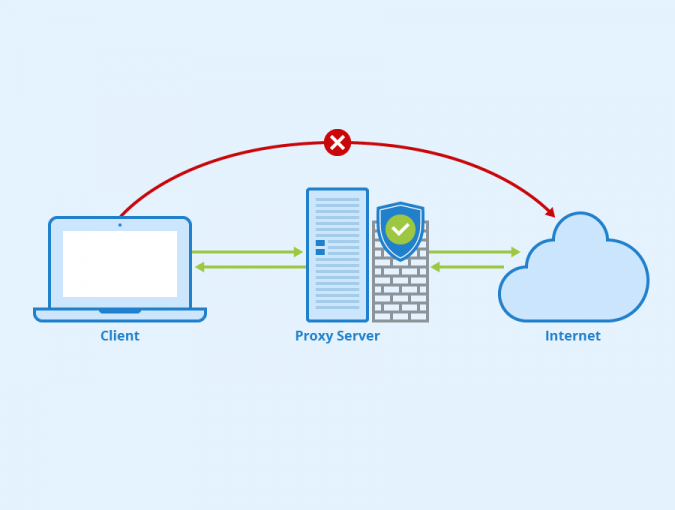
\includegraphics[width=0.6\textwidth]{obrazky-figures/Proxy-Server.png}
	\caption{Proxy Server. Autor: Seobility. License: \href{https://creativecommons.org/licenses/by-sa/4.0/deed.en}{CC BY-SA 4.0}. Bylo převzato z webu: \href{https://www.seobility.net/en/wiki/Proxy_Server}{https://www.seobility.net/en/wiki/Proxy\_Server}}
\end{figure}

Všechna zařízení připojená k internetu mají svou vlastní jedinečnou adresu internetového protokolu. Podle této IP adresy jsou v síti rozpoznána a používají ji ke komunikaci a určení správného cíle pro přenos dat. Adresa je rovněž důležitá pro fungování proxy serveru~\cite{proxy1}. 
Proxy server je jako počítač s vlastní IP adresou~\cite{proxy2}. Komunikace probíhá v následujících fázích:

\begin{enumerate}
  \item{Uživatel odešle na internet požadavek, který je odeslán proxy serveru. Tento~požadavek je následně přečten a interpretován~\cite{proxy1}.}
  \item{Proxy server předá požadavek cílovému serveru. Při předávání požadavku uvede proxy server jako zdrojovou adresu svou IP adresu~\cite{proxy2}.}
  \item{Server zpracuje požadavek a odešle odpověď proxy serveru~\cite{proxy1}.}
  \item{Proxy server ověří data, změní jejich obsah nebo provede jiné úkoly, které mu byly přiděleny, a poté předá odpověď uživateli~\cite{proxy2}.}
\end{enumerate}

\section{Princip činnosti nástroje}
\label{princip}
\begin{figure}[H]
	\centering
	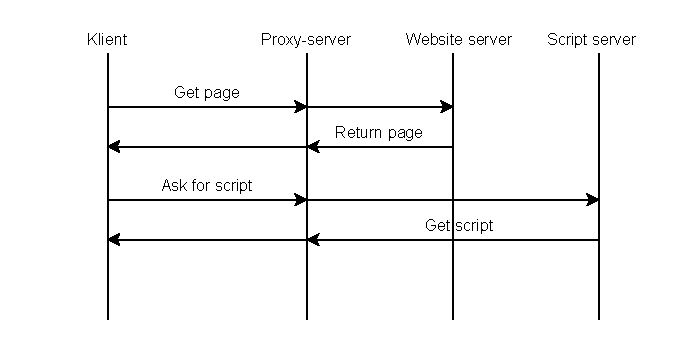
\includegraphics[width=0.9\textwidth]{obrazky-figures/diagram.pdf}
	\caption{Schéma komunikace mezi prohlížečem, proxy serverem a dalšími servery}
	\label{img:proxy}
\end{figure}

V této části podrobně popíšu, jak prohlížeč a servery komunikují při použití proxy serveru za účelem mé práce -- obejít blokátory marketingové, analytické a remarketingové skripty. 

Je třeba zdůraznit, že očekávané nasazení proxy serveru se předpokládá v síti serveru webové stránky. 

Na obrázku~\ref{img:proxy} je znázorněna zjednodušená verze komunikace, kterou podrobněji popíšu níže.

Při otevření webové stránky odešle prohlížeč klienta požadavek na načtení stránky na server webové stránky. Pokud je použit proxy server je požadavek nejprve přijat jím a přesměrován na požadovaný server. Server vrátí proxy serveru odpověď s obsahem stránky, která může obsahovat skripty, jež by mohly být v budoucnu potenciálně blokovány prohlížečem klienta. V této fázi musí proxy server zamaskovat adresy URL skriptů a vrátit klientovi upravený obsah. Pod pojmem 'maska' mám na mysli novou URL adresu, která nahradí předchozí, aby nedocházelo k blokování. 

Po přijetí obsahu prohlížeč odešle požadavek na stažení skriptu pomocí maskované adresy URL. Proxy server jej přijme, rozpozná a obrátí se na svůj keš. Pokud má keš kopii požadovaného skriptu, proxy server ji vrátí prohlížeči, ale pokud ji nemá, proxy server odešle požadavek na původní server skriptu, aby ji získal. Poté uloží kopii do svého keše pro další použití a skript vrátí klientovi. 

Výsledkem je, že se skript na straně klienta načte bez jakýchkoli omezení, aniž by byl blokován, a začne shromažďovat data.


\subsection*{Důležité aspekty komunikace}
\label{sub:4:aspekty}

Nyní se blíže podívám na aspekty, kterým je třeba věnovat pozornost při implementaci proxy serveru. Dosavadní popis komunikace byl poměrně zjednodušený a hlubší pohled na jednotlivé kroky a procesy odhalí místa, která se mohou potenciálně stát problémem a nejsou hned zřejmá. 

Jedním z těchto aspektů je server, ke kterému skript přistupuje za účelem stahování a výměny informací. Obvykle to není jen jeden server, jak je znázorněno na obrázku~\ref{img:proxy}, ale několik. Kromě serveru, ze kterého se stahuje samotný skript, mohou být požadavky zasílány různým serverům pro různé úrovně zpracování a použití dat. Takovým příkladem je server Google Analytics a marketingový a remarketingový server Google Ads, protože skript poskytnutý společností Google umožňuje přenášet shromážděná data do různých služeb Google~\cite{webSiteTag}.

Jinými slovy, i jednoduchý analytický skript společnosti Google bez dalších funkcí vyžaduje odeslání požadavků na nejméně dva servery pro stažení a přenos informací. Složitější skript integrovaný do několika služeb Google bude komunikovat s více doménami, což je třeba zohlednit při implementaci proxy serveru.

Problémem budou požadavky na související služby Google, kam budou odesílána data shromážděná z webu. Pokud byly první požadavky na Google Tag Manager zamaskované a mohly obejít blokování, pak budou následné požadavky na marketingové a analytické servery na přenos shromážděných dat blokovány a data nebudou moci dosáhnout svého koncového bodu. 

Jedním z řešení tohoto problému je změna koncového bodu pro odesílání shromážděných informací. Místo přímého odesílání na server Google Analytics nebo Google Ads můžete požadavek přesměrovat na adresu vytvořeného proxy serveru. To lze provést několika způsoby: prostřednictvím nastavení ve vlastním účtu Google Tag Manager nebo přidáním parametru do samotného skriptu. Při změně skriptu je třeba vložit pole \texttt{transport\_url}, jehož hodnotou bude adresa URL proxy serveru:
\begin{lstlisting}[caption=Skript pro změnu cílového serveru, label=transport-url]
gtag('config', 'G-XXXXX', {
  transport_url: 'https://example.com'
});
\end{lstlisting}

Tímto způsobem nebude požadavek zablokován a data budou odeslána na proxy server, který je následně předá analytickému nebo marketingovému serveru~\cite{endpoint}.

\bigskip

Maskování adres URL je jednou z nejdůležitějších částí práce mého proxy serveru a právě na něm bude založeno obcházení blokátoru. Pro úspěšné obejití blokace je třeba, aby program ke změně URL přistupoval kompetentně. Nová adresa URL nesmí způsobit podezření blokátoru, takže by neměla obsahovat známé vzory, jako jsou ty ze seznamů EasyPrivacy nebo EasyList, které budou blokovány, nebo nežádoucí slova. Příklady nežádoucích slov jsou např: \texttt{track}, \texttt{pixel} nebo \texttt{ad}, které budou detekovány jako podezřelé a zablokovány~\cite{ad}. 

Existuje několik přístupů k vytvoření maskované adresy URL. Níže stručně popíšu některé z těchto metod, jejich výhody a nevýhody.

\subsubsection{Kódování Base64}
Kódování Base64 je způsob, jakým jsou binární data reprezentována jako řetězec znaků. Princip fungování je následující:
\bigskip
\begin{itemize}
  \item{Vezme se vstupní řetězec, například URL, a převede se na binární data.}
  \item{Tato binární data jsou poté rozdělena do bloků po 6 bitech.}
  \item{Každá taková část odpovídá znaku z tabulky Base64.}
\end{itemize}
U URL se to používá v několika případech. Za prvé, když potřebujete do URL bezpečně vložit parametry. Tedy bez použití znaků, které by mohly způsobit problémy v segmentech cesty URL nebo v jejích parametrech. Ve druhém případě se tato metoda používá k ukrytí adresy URL, aby ji prohlížeč v kódu nerozpoznal a vnímal ji jako řetězec, a pouze jejím dekódováním ji bylo možné načíst~\cite{base64}.

\textbf{Výhody:} kompletní maskování adres. URL můžete získat zpět pouze dekódováním, tj. pouze proxy server bude vědět, co má dekódovat, a bude schopen získat adresu zpět. Navíc Java skript, na kterém bude proxy server napsán, má vestavěné funkce pro kódování a dekódování Base64, což zjednodušuje použití této metody~\cite{base64Git}.

\textbf{Nevýhody:} prohlížeč neuvidí adresu URL v maskovaném řetězci, tj. neprovede požadavek na tuto adresu. Další nevýhodou je, že velikost adresy URL se po zakódování mnohonásobně zvětší~\cite{base64Len}.

V případě mé práce není vyžadováno úplné maskování adresy URL, protože prohlížeč by měl v řetězci vidět adresu, na kterou má být požadavek odeslán. Je však možné použít kódování Base64 k maskování částí adresy URL, jako je cesta nebo parametry atd.

\subsubsection*{Hashing}
Hašování je proces převodu vstupní hodnoty, v případě mé práce zejména URL, na řetězec pevné délky nazývaný hash nebo digest. Nejběžnější použití hašování je při vytváření hašovacích tabulek. Hašovací tabulka ukládá dvojice hodnot na jejich indexy, což jsou hašovací hodnoty prvků. Mezi hašovací algoritmy patří: MD5, SHA-2, SHA-3~\cite{hash}. 

\textbf{Výhody:} bude mít výstupní šifrový text pevnou délku bez ohledu na velikost vstupní hodnoty. Šifrový text adresy URL nebude obsahovat žádná viditelná slova nebo vzory, které by blokátor mohl použít k filtrování adresy URL.

\textbf{Nevýhody:} hlavní nevýhodou je nevratnost procesu. Z haše nelze obnovit původní data, a tedy ani získat zpět původní adresu URL. Hašováním se celá adresa URL změní na běžný řetězec znaků, a proto ji prohlížeč nerozpozná jako adresu.

Bez drobné úpravy by se tato metoda neměla používat pro . Pokud na proxy serveru uložíte shodu mezi vstupními daty a jejich hash, bude možné získat originál ze zašifrované adresy URL. Stejně jako v případě metody Base64-encoding je však hašování možné pouze pro část adresy URL, nikoli pro celou adresu URL.

\subsubsection*{URL Shortening}
URL Shortening je proces přeměny dlouhých a složitých odkazů na krátké. Tato metoda se používá k vytvoření dokonalejších adres URL, které se snadno zapamatují a sdílejí~\cite{urlshort}. Pomocí nástroje pro zkracování adres URL se vytvoří zkrácená verze adresy URL, která vede na stejný cíl jako původní adresa URL. Funguje to následovně: zkrácený odkaz vede na server, který uchovává korespondenci mezi zkrácenou a dlouhou adresou URL, a po přijetí původní adresy URL je na tuto adresu přesměrován \cite{urlshortJS}. K vytvoření krátkých odkazů můžete použít známé služby, jako jsou Buff.ly, TinyURL, Bitly a další \cite{urlshort}. Nebo si můžete zkracovač URL vytvořit sami v programu. V případě mé práce potřebuji, aby proxy server generoval krátké adresy URL sám \cite{urlshortJS}. 

\textbf{Výhody:} dlouhý odkaz s klíčovými slovy a vzory je převeden na zkrácený a neutrální odkaz, u kterého je menší pravděpodobnost zablokování. Možnost integrovat metodu do proxy serveru. A také malá velikost vytvořeného krátkého odkazu, který nezabere mnoho místa a paměti.

\textbf{Nevýhody:} je třeba uložit do paměti nebo do databáze shodu mezi krátkým odkazem a původní adresou URL.

Tato metoda nevyžaduje žádnou další logiku, která by byla integrována do mé aplikace, protože sama provede všechny potřebné funkce -- maskování adresy URL a po nalezení původní adresy URL v mapě korespondence bude použita pro proxy.
\bigskip

Metodu maskování URL zvolím ve fázi implementace proxy serveru. V praxi tak budu moci zjistit, jak snadné bude jednotlivé adresy integrovat do vytvořeného proxy serveru a zda maskované URL budou schopny blokátor obejít. Na základě účinnosti bude vybrána konečná verze metody maskování URL.



\chapter{Implementace programu}
\label{ch:5}

V této části bude popsána implementace proxy serveru, který umožní obejít blokování analytických, marketingových a remarketingových skriptů v prohlížeči. Podrobně budou rozebrány použité technologie, architektura řešení, klíčové funkce nebo struktury v kódu, které budou zodpovědné za určité fáze proxy serveru, jako je zpracování požadavků a odpovědí, maskování adres URL, ukládání dat do mezipaměti atd. Zmíněny budou také potíže, na které jsem se při implementaci nástroje narazila, a jejich řešení. Závěrečným cílem této části bude prokázat funkčnost navrženého přístupu v kapitole~\ref{ch:4}, případně s drobnými odchylkami od původního plánu.

\section{Vybrané technologie}
Pro implementaci proxy serveru byl zvolen framework \textbf{Node.js}. 
Node.js je multiplatformní prostředí a knihovna s otevřeným zdrojovým kódem, která se používá ke spouštění webových aplikací a serverů mimo prohlížeč uživatele. Je zdarma a v dnešní době je aktuální, protože je neustále upravován a vylepšován celosvětovou komunitou vývojářů. Pro upřesnění, Node.js není framework nebo knihovna, ale spíše běhové prostředí JavaScriptu. Toto prostředí obsahuje webová API, která mohou vývojáři využít k vytváření kódu. Kód je následně analyzován a zpracován JavaScriptovým enginem~\cite{nodejs}.

Node.js je tedy flexibilní a lze jej nasadit jak lokálně, tak v libovolné cloudové službě. Díky vestavěným možnostem a existujícím knihovnám je vhodný také pro práci s požadavky HTTP a pro vytvoření proxy serveru.
\bigskip

Nyní se blíže podívám na knihovny Node.js, jejich funkce a vlastnosti.

\textbf{http-proxy}~\cite{http-proxy} je knihovna, která umožňuje programovat proxy servery HTTP podporující webové sokety. Slouží ke zpracování a předávání požadavků na jiné servery a je základem proxy serveru v rámci této práce.

\textbf{http}~\cite{http} je knihovna pro vytváření serverů a klientů HTTP. Tento modul umožňuje zpracovávat požadavky mezi klientem a serverem prostřednictvím protokolu HTTP. V rámci této práce bude využito tuto knihovnu k vytvoření základního serveru HTTP, který bude přijímat požadavky z prohlížeče.

\textbf{https}~\cite{https} -- knihovna, která se v mé práci používá k odesílání požadavků HTTPS.

\textbf{fs}~\cite{fs} -- knihovna pro práci s lokálním souborovým systémem. Tento modul slouží k~ukládání nebo čtení skriptů.

\textbf{zlib}~\cite{zlib} -- knihovna, která poskytuje kompresi a dekompresi dat implementovanou pomocí Gzip, Deflate/Inflate, Brotli a Zstd.

\textbf{path}~\cite{path} -- modul, který umožňuje práci s cestami k souborům a adresářům. Jeho prostřednictvím lze bezpečně kombinovat cesty k souborům.

\textbf{url}~\cite{url} -- modul, který poskytuje utilitky pro rozlišení a parsování URL adres.

\section{Logika proxy serveru}

Hlavní soubor, který je základem proxy serveru, se nazývá \emph{index.js}. Samotný proxy server je vytvořen pomocí příkazu \texttt{createProxyServer(options)} z knihovny \texttt{http-proxy}. Pro plnou kontrolu nad odpověďmi, které proxy server přijme od cílových serverů, používám volbu \texttt{selfHandleResponse: true}.
Vytvořený objekt proxy ještě nepředstavuje webový server. Aby byl vytvořen a spuštěn server, který bude přijímat požadavky z prohlížeče, použijí se následující dvě funkce z knihovny \texttt{http}~\cite{http-proxy}:

\begin{itemize}
    \item \texttt{http.createServer((req, res) => \{\})} -- vytvoří HTTP-server~\cite{http}.
    \item \texttt{server.listen(port)} -- spustí vytvořený server na zadaném portu~\cite{http}.
\end{itemize}

Všechny požadavky, s výjimkou těch, které byly maskovány, proxy server přijme a proxuje pomocí metody \verb|proxy.web(req, res, { target:'http://domain:port'})|~\cite{http-proxy}. Kde \texttt{domain:port} je adresa a port webového serveru, na který jsou přesměrovány dotazy související se načítáním a fungováním stránky.

Dále je přidána obsluha události \texttt{proxyRes}, která přijímá odpovědi z cílových serverů a umožňuje je modifikovat~\cite{http-proxy}. Základní funkce, tedy příjem, přesměrování požadavků, změna odpovědi a oddělení běžných požadavků od maskovaných, jsou tedy realizovány metodami a funkcemi, které jsem popsala výše v této sekce. 

Upozorňuji, že v mé verzi proxy serveru je pro provedení funkcí v něm zabudovaných nutné, aby uživatelé přecházeli na adresu, na které běží samotný proxy server, nikoliv webový server. 

Kromě toho se ihned po spuštění proxy serveru vyvolá funkce \texttt{downloadEasyPrivacy()}, která se nachází v souboru \texttt{maskUrl.js}. Hlavním úkolem této funkce je získat seznam EasyPrivacy a uložit soubor se seznamem do lokální složky proxy serveru \texttt{filter\_list}. Pokud je tato složka prázdná, proxy iniciuje HTPPS požadavek typu GET na oficiální URL adresu, na které se nachází aktuální verze seznamu EasyPrivacy~\cite{easyPrivacy}. Po úspěšném navázání spojení a obdržení odpovědi s obsahem proxy server načte příchozí datový tok a uloží jej do vytvořeného souboru \verb|'easyprivacy.txt'|.

Všechny stavové kódy, které bylo nutné ručně generovat v odpovědích od proxy serveru do prohlížeče uživatele, jsem vybrala na základě online zdroje, který obsahoval podrobnou příručku HTTP stavových kódů~\cite{statusCode}. 

\section{Zpracování odpovědi serveru}

V této sekci jsou popsány konkrétní akce proxy serveru v obsluze události \texttt{proxyRes}~\cite{http-proxy}:
\begin{lstlisting}[caption=Event 'proxyRes']
proxy.on('proxyRes', (proxyRes, req, res) => {
  // server response handling
});
\end{lstlisting}
a obtížím, které byly zaznamenány v průběhu implementace.

Hlavním úkolem popsané funkce je identifikovat ze všech odpovědí serveru tu, která obsahuje HTML stránku, a modifikovat ji. Všechny ostatní typy obsahu v odpovědi, pokud nejde o \texttt{text/html}, nebudou zasahovány a budou předány prohlížeči v takové podobě, v~jaké byly přijaty ze serveru. Dalším krokem je sestavení odpovědi do jednoho bloku, jelikož rozsáhlá odpověď může být odeslána po částech. Jakmile server kompletně odešle odpověď, nastane událost \texttt{'end'} a lze pracovat s proměnnou, která bude obsahovat tuto odpověď.

V některých případech může server vrátit komprimovanou odpověď, kterou nelze přímo upravit. Proto byla následně přidána dekomprese odpovědi za předpokladu, že byla uvedena v hlavičce \texttt{content-encoding}. V proxy serveru jsem zohlednila možnost, že mohou být použity následující formáty komprese: \texttt{gzip}, \texttt{deflate} a \texttt{br}, nebo odpověď nebyla zakódována vůbec~\cite{encoding}.

Následně je odpověď ze serveru připravena k modifikaci, která probíhá ve volané funkci \texttt{modifyHTML}. V rámci této funkce se nejprve vyhledá adresa URL, která se obvykle používá k načtení skriptu, který spouští {\it tag} na webové stránce (viz výpis~\ref{google-tag-script}). Pokud je nalezena shoda, proxy server samostatně zašle požadavek na cílový server pomocí nalezené adresy URL. Z odpovědi získaný skript je dále uložen lokálně. Vzhledem k tomu, že na jedné  webové stránce může být umístěn pouze jeden {\it tag}, bude existovat pouze jedna URL adresa. Uložený skript se následně projde funkcí \texttt{maskUrlInScript}, která zamaskuje adresy URL, které mohou způsobit vznik podezření ze strany blokátoru (viz sekce~\ref{sec:5:mask}). Po úpravě staženého skriptu proxy-server dále pracuje s HTML kódem stránky. Funkce \texttt{maskUrlInHTML} se volá ze souboru \texttt{maskUrl.js}. Tato funkce znovu najde URL adresu v kódu HTML a zamaskuje ji následujícím způsobem:
\begin{enumerate}
    \item Řetězec z URL, bez uvozovek, je zahešován pomocí algoritmu \texttt{'md5'}. Z možností maskování, které jsem popsala v sekci~\ref{princip}, jsem zvolila hašování, které je zcela základní, existuje pro něj řada algoritmů a je možné ho použít v \textbf{Node.js} pomocí knihovny \textbf{crypto} \cite{crypto}. Algoritmus \texttt{'md5'} byl zvolen, jelikož generuje jeden z nejkratších hešů co do délky ve srovnání s ostatními algoritmy. Vzhledem k tomu, že hešování v mé práci slouží pouze k maskování, nikoli k zabezpečení, je menší velikost hešů více výhodou než nevýhodou~\cite{md5}.
    \item Dalším krokem je uložení mapování mezi URL adresou a z ní vygenerovaným hešem do mapy \texttt{urlMap}. Důvodem je to, že algoritmus hešování je nevratný a dané URL může být v budoucnu potřeba.
    \item Původní URL je teď nahrazeno následujícím:\\
    \texttt{http://domainOfYourProxy/proxy-script/hash}. Je důležité použít protokol HTTP, protože můj proxy server je zaměřen na přijímání HTTP-požadavků. Aby bylo možné plně zachytit HTTPS požadavky a mít přístup k úplné URL adrese a hlavičkám, což budu potřebovat při přijímání maskovaných požadavků, musí být proxy server důvěryhodným certifikátem v prohlížeči klienta. Na rozdíl od HTTP požadavků, jejichž provoz je pro proxy server transparentní, což umožňuje přístup ke všem potřebným údajům požadavku~\cite{mitm}. S ohledem na to jsem se rozhodla maskované požadavky přenášet protokolem HTTP, protože tak může proxy server provádět potřebné zpracování bez složité konfigurace šifrování a nastavení potřebných certifikátů. Zároveň jsem zkontrolovala, že část cesty URL \texttt{proxy-script} se neobjevuje ani v seznamu filtrů EasyPrivacy, ani v seznamu EasyList.
\end{enumerate}

Následně změním hlavičku \texttt{content-length} na skutečnou velikost upraveného HTML kódu a odstraním hlavičku \texttt{content-encoding}, aby prohlížeč neočekával komprimovanou odpověď. Posledním krokem v obsluze události proxyRes je odeslání upraveného HTML kódu do prohlížeče uživatele. 

Tímto způsobem je proxy server připraven přijímat zamaskované požadavky z prohlížeče a předávat klientovi skript přijatý ze serveru Google Tag Manager.
\bigskip


\section{Maskování URL ve skriptu přijatém ze serveru Google Tag Manager}
\label{sec:5:mask}

V návrhu jsem popsala následující algoritmus pro maskování požadavků, které {\it tag} odesílá souvisejícím službám Google: změna koncového bodu odesílání dat na adresu proxy serveru (viz podsekce~\ref{sub:4:aspekty}). Během implementace však byl zjištěn problém, kvůli kterému bylo nutné změnit postup. Problém byl způsoben tím, že ne všechny požadavky související s {\it tagem} byly tímto mechanismem maskovány a zachyceny. Například následující změna v koncového bodu cesty, která je uvedena v výpisu~\ref{transport-url}, by zachytila pouze požadavky směřující do služby Google Analytics, protože identifikátor začínající písmenem \texttt{G-} odkazuje na účty vytvořené v Google Analytics~\cite{idGoogle}. Kromě toho však může {\it tag} posílat opakované požadavky do Google Tag Manageru, což jsem v praxi zjistila při prohlížení souboru \texttt{gtag.js}. Metoda popsaná v návrhu by však takové požadavky nezamaskovala, což by mohlo způsobit selhání nebo nesprávné fungování skriptu.

Z tohoto důvodu tuto variantu jsem považovala za nevhodnou a začala jsem hledat jiné řešení. Po podrobném prostudování výsledného skriptu \texttt{gtag.js} jsem došla k závěru, že v~tomto skriptu jsou generovány všechny adresy URL na které může {\it tag} odesílat požadavky (tj. požadavky související s {\it tagem}). Skript obsahuje fragmenty URL, kde základ, tj. doména a někdy i základní cesta, je vložen do kódu jako řetězec a zbytek URL je generován dynamicky -- reprezentován jako proměnné. V závislosti na konfiguraci {\it tagu} tak může \texttt{gtag.js} použít jeden z řetězců, které tvoří URL do cílového serveru, na který budou shromážděná data odeslána. Nakonec jsem přišla na metodu, při které budu maskovat adresy URL, které mohou být blokovány v samotném souboru \texttt{gtag.js}, než je předám prohlížeči uživatele. V~této části budou popsány technické podrobnosti implementace tohoto přístupu.

Hlavní funkce, která modifikuje skript předaný v argumentech, se nachází v souboru \texttt{maskUrl.js} a nazývá se \texttt{maskUrlInScript(content)}. Argumentem funkce je předaný obsah skriptu, ve kterém má být maskováno URL. Funkce nejprve načte soubor \texttt{easyprivacy.txt}, který byl stažen do adresáře proxy serveru z oficiálního zdroje~\cite{easyPrivacy}. Vzhledem k tomu, že seznam EasyPrivacy je zaměřen více na sledování prvků na stránce, rozhodla jsem se, že bude vhodnější použít jej k vyhledání URL, které je třeba zamaskovat.

Algoritmus prochází řádky seznamu EasyPrivacy a kontroluje, zda splňují podmínku, která je kontrolována ve funkci \texttt{domainLine(line)}. Tímto způsobem vyberu pouze řádky, které obsahují URL domény nebo části domény. Toto rozhodnutí jsem učinila s ohledem na to, že plná podpora všech možných syntaktických pravidel by vyžadovala složitý parser a hlubší analýzu kódu \texttt{gtag.js}, což není hlavním cílem mé práce. To byl důvod, proč jsem se zaměřila pouze na vyhledávání adres URL, které obsahují domény ze seznamu EasyPrivacy. Tento přístup stále umožňuje zahrnout značný počet potenciálně blokovaných požadavků, aniž bychom se museli uchýlit k úplnému parsování pravidel. Hlavním cílem mé práce je tedy prokázat účinnost použití metody maskování URL k obcházení blokátorů.

Funkce \texttt{domainLine(line)} kontroluje, zda má řetězec jeden z následujících typů podoby:
\begin{itemize}
    \item Řetězec začíná znakem \texttt{||}, který je explicitním indikátorem domény.
    \item Řetězec začíná znakem \texttt{.} a obsahuje znak \texttt{/} a dále se kontroluje, zda řetězec odpovídá regulárnímu výrazu: \verb|/^\.[.a-zA-Z0-9-]+\/.*/|. Tento výraz odpovídá řetězcům, které začínají tečkou, za níž následuje kombinace znaků přípustných pro doménu, znak \texttt{/} a jakýkoli následný obsah. Protože objem kontrolovaných řetězců je velmi velký, byla z důvodu optimalizace přidána kontrola na \texttt{line.includes('/')},
 protože pokud řetězec tento znak neobsahuje, regulární výraz se neprovede, což ušetří čas. 
\end{itemize}

Pokud řetězec projde kontrolou a spadá pod výše uvedenou variantu, zavolá se funkce \texttt{getDomain(line)}, která z řetězce odstraní syntaktická pravidla a ponechá čistý řetězec části URL. V prvním kroku se odstraní znaky \texttt{||} ze začátku, v dalším kroku se hledá nejbližší shoda s jedním z následujících znaků: \verb|^|, \verb|$|,  nebo \verb|?|.  Následně jsou odříznuty: parametry cesty, tj. vše za znakem \texttt{?}, včetně něj; pravidla používaná pro typy dotazů, tj. vše za znakem \verb|$|; a vše za oddělovačem \verb|^|, opět včetně něj. Ve většině případů jsou parametry URL cesty v souboru \texttt{gtag js}, jak jsem se zmínila výše, tvořeny dynamicky, proto by bylo zbytečné je hledat jako vložený řetězec. Ponechávám tedy pouze tu část pravidla, kterou by bylo reálné ve skriptu najít, a zamaskovat.

Nyní je řetězec připraven pro vyhledávání shod ve skriptu. Tento proces probíhá ve funkci \texttt{replaceDomain(content, domain)} a je rozdělen na dvě části, dvě možnosti nalezení shody a jejího nahrazení.

\textbf{První varianta:} vyhledá řetězce, které mají proměnnou v subdoméně. Takové řetězce je třeba správně zamaskovat, aniž by se změnila část, která obsahuje vložení proměnné, proto jsem ji vyčlenila do samostatné varianty. Mým cílem bylo použít regulární výraz k nalezení shody a následně pomocí skupin zachycení zamaskovat nalezený řetězec. Regulární výraz první varianty je následující:

\begin{lstlisting}[caption=Regulární výraz]
  (["'])                            
  https:\/\/                        
  (
    ["']\\+[^+]+\\+["']\\.?           
    |["']\\+\\([^)]+\\)\\+["']\\.?      
    |\\{[^}]+\\}\\.?                   
  )
  (?:${searchPart})             
  ([/?][^"']*)?                    
  (["']) 
\end{lstlisting}

\begin{itemize}
    \item \verb|(["'])|  -- capture group typu uvozovek.
    \item \verb|https:\/\/| -- hledající shodu s \texttt{https://}.
    \item \verb!(["']\\+[^+]+\\+["']\\.?|["']\\+\\([^)]+\\)\\+["']\\.?|\\{[^}]+\\}\\.?)! -- druhá capture group hledající proměnné v subdoméně. V rámci tohoto zkoumání byly nalezeny tři hlavní typy vkládání proměnných, které byly použity jako základ pro vyhledávání. \verb!["']\\+[^+]+\\+["']\\.?! zachycuje zřetězení tohoto typu proměnné: \texttt{"+a+"}, stejně jako případnou tečku na konci. \verb!["']\\+\\([^)]+\\)\\+["']\\.?! je regulární výraz, který také zachycuje zřetězení, ale proměnné se složitější strukturou, například \texttt{"+(a?a+".":"")+"}. A konečný regulární výraz \verb!\\{[^}]+\}\\.?! zachycuje proměnnou ve stylu šablonování -- \verb|{var}|. 
    \item \verb!(?:${searchPart})! -- je nezachycující skupina, která obsahuje řetězec získaný ze seznamu EasyPrivacy.
    \item \verb!([/?][^"']*)?! -- nepovinná zachycující skupina zbytku URL. 
\end{itemize}

Pokud najdu shodu, řetězec ve skriptu zamaskuju. Část získaná ze seznamu EasyPrivacy je zahešována a přidána do mapy \texttt{urlMap} a původní URL je upravena následujícím způsobem: typ protokolu, doména a základní cesta jsou změněny na ty, které povedou k proxy serveru, a proměnná spolu s hešem a zbytkem URL (pokud byla) je vložena jako pokračování. Nová URL tedy vypadá např. takto:

\verb|http://domainOfProxy/proxy-send/variable~hash/restOfPath|


\textbf{Druhá varianta:} druhá varianta má podobný regulární výraz, ale bere v úvahu URL, které nemají v doméně proměnnou. Popíšu pouze tu část regulárního výrazu, která se liší od první varianty:
\begin{itemize}
    \item \verb|([^.+"'{}()]*\\.?)?| -- volitelná skupina zachycující subdoménu.
\end{itemize}

Může se stát, že výsledný řetězec ze seznamu EasyPrivacy bude obsahovat pouze hlavní doménu a já potřebuji zachytit a přenést subdoménu, abych byla schopna rekonstruovat původní URL po heši. Vzhledem k tomu, že vytvořená zamaskovaná URL bude mít doménu proxy serveru, původní doménu přesunu do segmentu její cesty. Proto je pro mě důležité pomocí zachycení skupiny regulárního výrazu získat původní subdoménu, pokud existuje, a zachovat ji v segmentu cesty nové URL. Tímto způsobem při odmaskování budu schopna přesně obnovit počáteční URL adresu, aniž bych ztratila jakoukoli její část a zachovala jejich pořadí.

Když je tedy nalezena shoda s jedním z regulárních výrazů, požadovaný URL řetězec se zamaskuje a proces se opakuje pro další pravidlo v seznamu EasyPrivacy.

Při testování bylo zjištěno, že pouze výše popsaná změna nestačí k obejití všech blokování. V EasyPrivacy bylo hodně pravidel souvisejících se segmentem cesty \texttt{/collect}, které v mé předchozí verzi nebyly zohledněny. Kromě toho bylo při testování s odesíláním shromážděných dat do Google Analytics zjištěno, že požadavek je blokován kvůli specifické kombinaci parametrů URL, která je v EasyPrivacy popsána jako \verb|?v=2&tid=G-$~third-party|. Ale jak jsem již několikrát zmiňovala, ve skriptu typu \texttt{gtag.js} jsou parametry URL ve většině případů generovány dynamicky pomocí proměnných, takže by bylo obtížné najít dané pravidlo ve formě řetězce. Podařilo se mi však najít proměnnou, která odpovídala verzi uvedené v parametrech \texttt{v=2}, což pomohlo při maskování. Tímto způsobem byla přidána funkce, která najde všechny \texttt{/collect}, které se nacházejí v řetězci, jejichž doména již byla změněna na doménu proxy, a nahradí je slovem \texttt{/proxy-get}, které není součástí pravidel EasyPrivacy a EasyList. Tuto slovní spojení jsem zvolila, aby na jedné straně nevzbuzovalo podezření blokátorů a na druhé straně bylo snadno identifikovatelné proxy serverem v rámci analýzy přijatých požadavků. Tento přístup pomůže v budoucnu odlišit maskované požadavky od ostatních a zároveň obejít blokátor obsahu, protože \texttt{proxy-get} není součástí pravidel dvou základních seznamů filtrování. Dalším krokem byla změna hodnoty proměnné verze. 

Tyto změny umožnily výrazně snížit počet blokovaných požadavků. Ačkoli navrhovaný přístup nezahrnuje maskování všech možných případů a nezaručuje absolutní obcházení blokátoru, demonstruje možnost realizace obcházení blokátoru pomocí proxy serveru, který maskuje URL. Za předpokladu úplného parsování pravidel EasyPrivacy a hlubší analýzy skriptu \texttt{gtag.js} může být popsané řešení dopracováno až k prakticky úplnému obejití blokátorů. Realizace podobného mechanismu však vyžaduje mnohem více času a zdrojů, což přesahuje rámec této práce.

\section{Přijímání požadavků z prohlížeče}
Nyní bude podrobněji popsáno práci vytvořeného HTTP serveru, který přijímá požadavky z prohlížeče. Jeho základní struktura vypadá následovně:
\bigskip
\bigskip
\begin{lstlisting}[caption=Function that receives browser requests]
const server = http.createServer((req, res) => {
  if (req.url.includes('proxy-send')) {
    // processing tag requests for sending collected information
    return;
  }
  
  if (req.url.includes('proxy-script')) {
    // processing requests for receiving scripts from Google Tag Manager
    return;
  }
  
  proxy.web(req, res, { target: 'http://domainOfWebsite' });
});
\end{lstlisting}
První dvě podmínky zpracovávají maskované požadavky přijaté z prohlížeče klienta, které jsem rozdělila na ty, které vyžadují získání skriptu z proxy keše, a ty, které vyžadují přesměrování požadavku na původní URL. Funkce \texttt{web} z knihovny \textbf{http-proxy} automaticky přeposílá všechny ostatní požadavky přes proxy.

Dále následuje podrobnější pohled na zpracování požadavku se segmentem \texttt{proxy-send} v cestě. Takové požadavky je nejprve nutné vrátit do původního formátu, což se provádí ve funkci \texttt{getOriginalUrl}, která je napsána v souboru \texttt{maskUrl.js}. Na začátku se URL získaná funkcí rozdělí na části, aby se oddělila heš od zbytku originální URL a také aby se z ní odstranila doména a základní cesta proxy serveru. V proměnné, která přijímá zbytek URL, se provede vrácení zamaskovaného \texttt{/collect} a verze 2, pokud jsou nalezeny vzory, kterými byly tyto části nahrazeny.

Kromě toho se z mapy shod pomocí haše získá původní část URL. Při maskování URL, které jsem popsala v sekci~\ref{sec:5:mask}, byly subdoména a heš umístěny v jednom segmentu cesty a odděleny znakem \verb|~|. Toto oddělení bylo navrženo pro snazší vyjmutí haše ze segmentu. Následně se všechny části URL znovu spojí a na začátek se vloží \texttt{https://}. Po získání zrekonstruované URL je důležité změnit doménu v \texttt{req.headers.host}, protože hlavičky budou předávány v požadavku do služeb Google a je důležité, aby se shodovaly se zrekonstruovanou URL. Dalším krokem je samostatné vytvoření HTTPS požadavku ke službám Google. Požadavek se připraví pomocí funkce \texttt{https.request(originalUrl, options, (googleRes))}, tělo požadavku, pokud existuje, se přenese později pomocí \texttt{req.pipe(googleReq)}. V požadavku: \texttt{originalUrl} je původní URL, která byla získána z maskované; \texttt{options}  je objekt s parametry: \texttt{method} a \texttt{headers}, předané z požadavku získaného z prohlížeče \cite{https}. \texttt{googleRes} je objekt odpovědi cílového serveru na daný požadavek. Kromě toho se po obdržení odpovědi provádí další kontrola jejího záhlaví \texttt{content-type}. Pokud odpověď obsahuje javascriptový kód, je třeba jej znovu zkontrolovat na přítomnost potenciálně blokovaných URL a zamaskovat je. Odpověď serveru v tomto případě není nutné ukládat do proxy keše, proto ji program shromažďuje po částech, v případě potřeby dekomprimuje a volá funkci \texttt{maskUrlInScript} (viz sekce \ref{sec:5:mask}). Poté je odpověď předána pomocí funkce \texttt{pipe} do objektu \texttt{res}, který se vrátí prohlížeči.

Dalším a posledním zpracováním zamaskované URL adresy je zpracování těch, které mají v cestě segment \texttt{proxy-script}. Tyto požadavky vyžadují vrácení skriptu uloženého v keši proxy serveru. V této fázi proxy vezme skript uložený u sebe a vrátí jej prohlížeči. Vzhledem k tomu, že pro jednu stránku je potřeba jeden takový skript pro fungování sledování na ní, nejsou problémy s rozlišením mezi skripty -- prohlížeč obdrží ten skript, který se v danou chvíli nachází v keši proxy.

\chapter{Testování}
\label{ch:6}

Tato kapitola práce bude věnována popisu procesu testování mnou implementovaného řešení, jehož účelem je zajistit účinné obejití mechanismů blokování analytických, marketingových a remarketingových skriptů. Hlavním cílem této fáze práce bylo praktické ověření funkčnosti mnou navrženého řešení a také zkoumání reakce programu při modelování různých testovacích scénářů. Konkrétně ověření mělo ukázat, zda jsou získané výsledky v~souladu s očekávanými, tj. s logikou fungování, která byla stanovena ve fázi návrhu proxy serveru. Kromě hlavního úkolu mělo testování ještě jednu důležitou funkci -- odhalení možných slabých míst v implementaci. Umožnilo identifikovat technická i logická omezení navrhovaného řešení, pomohlo odhalit nedostatky a také pomohlo vytvořit seznam aspektů, které vyžadují další optimalizaci a vylepšení. S cílem zajistit komplexní přístup k testování byly stanoveny klíčové oblasti a scénáře, ve kterých byl implementovaný proxy server použit. Mezi ně patří:

\begin{enumerate}
    \item Testování proxy serveru v přítomnosti různých blokátorů zabudovaných jako rozšíření v prohlížeči. Byly použity zejména nástroje, které pracují na základě seznamů blokovaných URL adres. Tímto způsobem se ověřuje adaptabilita proxy serveru na různé blokátory, které mohou být zapnuty na straně klienta v jeho prohlížeči.
    \item Hodnocení efektivity navrženého řešení při použití různých produktů společnosti Google souvisejících se sběrem analytických dat, realizací marketingových kampaní nebo remarketingem. V rámci tohoto směru byla analyzována schopnost systému zajistit správný přenos a zpracování dat i při práci blokátorů na straně klienta.
    \item Analýza chování programu v rámci webového prohlížeče s ohledem na různé možnosti ukládání do mezipaměti -- jak v případě, kdy lokální mezipaměť prohlížeče ukládá data získaná ze serverů, jako jsou například skripty, tak i v případě zcela čisté mezipaměti, tj. například při první návštěvě stránky klientem. To umožnilo vyhodnotit, jak stabilně řešení funguje v různých stavech klientského prohlížeče.
\end{enumerate}

\section{Základ pro testování}
V této části se soustředím na řadu technických aspektů souvisejících s testováním proxy serveru, který jsem implementovala. Zejména uvedu, že jako prostředí pro spuštění programu bylo použito \textbf{Node.js} verze v18.20.4. Instalace závislostí proběhla pomocí správce balíčků \textbf{npm} verze 9.9.3.

Prvním krokem přípravy na testování byla potřeba mít webový zdroj, ke kterému by bylo možné přistupovat za účelem instalace {\it tagu} a sledování požadavků odeslaných ze stránky. K tomuto účelu byl použit můj vlastní web, umístěný na univerzitním serveru \texttt{Merlin} a dostupný na URL adrese, která obsahuje mé osobní přihlašovací jméno. Webová stránka má poměrně jednoduchou strukturu: jedná se o klasickou jednostránkovou webovou stránku se souborem index.html, který obsahoval základní HTML obsah, odkaz na externí CSS soubor pro stylizaci a několik obrázků pro ilustrační účely.

Dalším důležitým krokem byla příprava testování reálných analytických, marketingových a remarketingových nástrojů. Za tímto účelem jsem vytvořila účty ve dvou hlavních službách společnosti Google, které se aktivně používají pro sběr analytických údajů a realizaci marketingových a remarketingových strategií -- Google Analytics a Google Ads. Tyto služby sloužily jako základ jak pro fázi výzkumu analytických, marketingových a remarketingových skriptů popsaných v kapitole~\ref{ch:2}, tak i nyní pro fázi testování. 

Následně jsem na webovou stránku přidála základní Google Tag, který jsem podrobně popsala v sekce~\ref{sec:2:analytics}. Během testování jsem jej připojila k jednomu z mnou dříve vytvořených účtů ve službách Google, což umožnilo spustit základní konfiguraci sledování chování uživatelů na webu, jako je prohlížení stránky, posouvání stránky až na konec a další. 

V počátečních fázích implementace a ověřování funkčnosti proxy serveru jsem zvolila nejjednodušší způsob testování, při kterém byl server spuštěn lokálně na mém počítači a nastavení systému bylo změněno tak, aby všechny externí HTTP požadavky z prohlížeče byly nejprve přesměrovány na spuštěný proxy server. Tento přístup sice umožňoval rychle provádět základní testy, ale nakonec se ukázal jako neúčinný a dokonce chybný z několika důvodů. Za prvé, v průběhu dalšího testování bylo zjištěno, že blokovače reklam, jako je uBlock Origin Lite, nepoužívají všechna pravidla blokování ze svého seznamu na požadavky, které jdou na doménu localhost, tj. jdou na lokální adresy. To snižuje spolehlivost výsledků testů. Za druhé, taková architektura neodpovídá realistickému scénáři použití. V praxi klientské prohlížeče nebudou měnit svá síťová nastavení, aby směrovaly provoz přes cizí proxy server. Správná implementace proxy naopak předpokládá jeho integraci na straně webové stránky. Tímto způsobem proxy neviditelně pro uživatele zachycuje a zpracovává požadavky, aniž by vyžadoval jakýkoli zásah do konfigurace prohlížeče klienta. Výsledkem bylo přesunutí a nasazení proxy serveru přímo na univerzitní server \texttt{Merlin}, což umožnilo vytvořit podmínky co nejblíže reálným.

Kromě toho jsem změnila některé standardní parametry konfigurace proxy serveru. Konkrétně jsem nastavila port \texttt{3000} jako port, na kterém měl proxy server pracovat. To znamená, že po spuštění je proxy server dostupný na adrese \texttt{http://merlin.fit.vutbr.cz:3000}. Kromě toho mám na serveru \texttt{Merlin} ve složce \texttt{WWW} umístěnou hlavní webovou stránku. Právě z této složky se odesílají statické zdroje, jako je kód HTML, styly CSS, obrázky a další, které jsou nezbytné pro správné zobrazení stránky v prohlížeči. Aby proxy mohl komunikovat s tímto obsahem, konkrétně přenášet požadavky prohlížeče na získání prvků stránky a vracet mu odpověď, vytvořila jsem jako cílový server -- Express server, který by se spouštěl společně s proxy a pracoval na portu \texttt{8080}. K tomu jsem do své implementované programy přidala modul \texttt{'express'} pomocí příkazu \texttt{npm install express} a následující kód:
\bigskip
\bigskip
\bigskip
\bigskip
\bigskip
\bigskip
\begin{lstlisting}[caption=Express server]
const express = require('express');

const app = express();

// Static files served from the WWW folder containing the page code
app.use(express.static(path.join(__dirname, '../WWW')));

// Express server running on port 8080
app.listen(8080);
\end{lstlisting}

Pro vytvoření takového serveru jsem vycházela z příkladů z oficiální dokumentace knihovny \texttt{express}~\cite{express} a její sekce o obsluze statických souborů~\cite{expressStatic}.

V tomto kódu se vytváří Express server \texttt{app}, který se spouští na portu \texttt{8080}. 

\verb|app.use(express.static(path.join(__dirname, '../WWW')));| -- odpovídá za obsluhu statických souborů ze složky~\texttt{WWW}, jako jsou obrázky, CSS styly, HTML kód a JavaScript kódy~\cite{expressStatic}.

Tímto způsobem, když na Express server přijdou požadavky na získání potřebných souborů, vezme je ze souboru~\texttt{WWW} a vrátí je proxy serveru. 

Pro přesměrování požadavků na Express server jsem změnila cílový server na

\noindent\texttt{'http://127.0.0.1:8080'} ve funkci~\texttt{proxy.web}, což vypadá následovně:

\begin{lstlisting}[caption=Function web]
proxy.web(req, res, { target: 'http://127.0.0.1:8080' });
\end{lstlisting}

V důsledku toho byly všechny požadavky přicházející na proxy dále přesměrovány na interní expres server, který naslouchal na portu \texttt{8080}. Tímto způsobem uživatel při přechodu na URL proxy serveru, tj. \texttt{http://merlin.fit.vutbr.cz:3000}, získal zobrazení mé stránky umístěné ve složce \texttt{WWW} na serveru \texttt{Merlin}.

Dalším krokem bylo změnit doménu maskovaných URL na doménu proxy serveru ve všech funkcích, ve kterých docházelo k úpravám potenciálně blokovaných URL.

Tímto způsobem byly všechny požadavky -- jak na základní obsah, tak maskované požadavky související s analytickými, marketingovými a remarketingovými aktivitami skriptů na webu -- směrovány přímo na spuštěný proxy server. To mi umožnilo mít plnou kontrolu nad jejich zpracováním a možnost modifikovat jak odpovědi serverů, tak samotné požadavky před jejich dalším předáním.

Nyní, když byla základní konfigurace potřebná pro testování nastavena a popsána v této sekci, je možné přejít k posouzení a popisu konkrétních testovacích scénářů, ve kterých předvedu fungování proxy v podmínkách co nejblíže reálnému provozu.

\section{Testování s různými blokátory}
\label{ch:6:testBlok}
V této sekci budu testovat a sledovat práci proxy serveru za přítomnosti různých rozšíření na straně klienta, která fungují jako blokátory založené na seznamech blokovaných URL adres. 

Jak již bylo uvedeno v předchozí sekci, v počáteční fázi testování jsem vložila přímo pod prvek \texttt{<head>} na své HTML stránce příslušný skript. Jedná se o základní skript zobrazený na výpisu~\ref{google-tag-script}, který plní roli základního sledování interakce uživatele s webem, na kterém je umístěn. Jako službu, jejíž interakci s {\it tagem} bude zachycovat a zpracovávat proxy server, jsem zvolila Google Analytics, účet v němž byl vytvořen na počáteční fázi výzkumu fungování analytických skriptů. Klíčovým cílem testování tohoto scénáře bylo ujistit se, že požadavky odeslané {\it tagem} z prohlížeče uživatele nejsou filtrovány ani v případě aktivního blokátoru. Jelikož hlavní funkcí vloženého {\it tagu} je sledovat akce uživatele na webu a následně předávat shromážděné údaje do připojených produktů Google, což je také základem interakce analytického serveru s webem, rozhodla jsem se pro testování použít Google Analytics. Tento výběr umožnil vytvořit scénář blízký reálnému použití a současně sledovat práci proxy serveru v kombinaci s použitím blokátorů na straně prohlížeče uživatele. Pro nastavení tohoto procesu jsem nejprve v konfiguraci {\it tagu} uvedla identifikátor svého účtu v Google Analytics, díky čemuž byly všechny shromážděné údaje odesílány přímo do mého účtu a zobrazovány v jeho přehledech.

\subsection*{uBlock Origin Lite}
Jako první blokovač pro testování jsem zvolila \textbf{uBlock Origin Lite}. Na začátku implementace proxy jsem používala verzi uBlock Origin, ale po nějaké době přestalo být rozšíření podporováno a musela jsem ho nahradit uBlock Origin Lite, který je obdobou běžného uBlock Origin. 

Samotné testování bylo prováděno v prohlížeči Google Chrome, který poskytuje nástroje pro monitorování síťové aktivity. Konkrétně pro prohlížení a analýzu všech požadavků a odpovědí byl použit vestavěný nástroj vývojáře, konkrétně jeho sekce \texttt{Network}, která umožňuje v reálném čase sledovat síťovou aktivitu stránky. Před přímým zahájením testování byla z paměti prohlížeče odstraněna veškerá mezipaměť, aby byly vytvořeny podmínky blízké situaci, kdy uživatel navštíví stránku poprvé. Tím se předešlo nesprávným výsledkům, které by mohly vzniknout v důsledku vlivu dříve uložených lokálních dat v prohlížeči.

Po spuštění proxy serveru na Merlinu, s otevřeným oknem Nástroje vývojáře a aktivním rozšířením uBlock Origin Lite v režimu základního blokování, byl proveden první test přechodu na stránku podle odkazu \texttt{http://merlin.fit.vutbr.cz:3000}.

\begin{figure}[H]
	\centering
	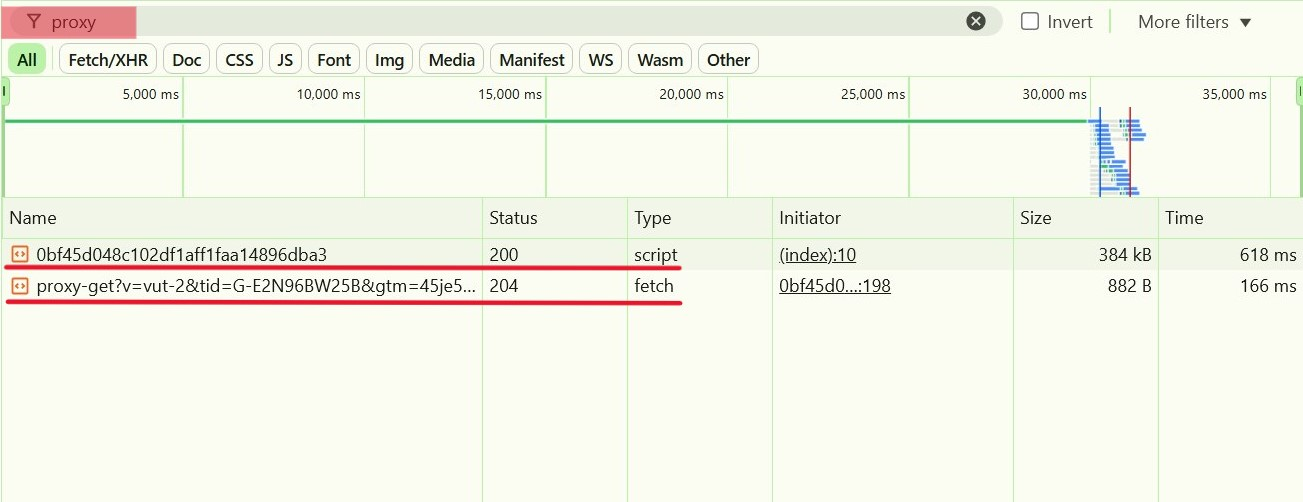
\includegraphics[width=1.0\textwidth]{obrazky-figures/reqTest1.jpg}
	\caption{Maskované požadavky}
    \label{img:maskedReq}
\end{figure}

Výsledkem testu bylo úspěšné obejití blokátoru dvou typů požadavků. První typ požadavků je požadavek odeslaný do Google Tag Manageru  za účelem získání skriptu \texttt{gtag.js}. Druhý typ požadavků je maskovaný požadavek, který měl odeslat Google Analytics shromážděné údaje o události, která popisovala jednu z interakcí uživatele se stránkou. V konkrétním případě tohoto testu byla odeslána událost \texttt{page\_view} -- návštěva stránky uživatelem. Jak je vidět na snímku obrazovky~\ref{img:maskedReq}, oba požadavky generované {\it tagem} a odeslané z prohlížeče uživatele úspěšně dosáhly cílového serveru. Žádný z požadavků nebyl blokován aktivním rozšířením pro filtrování uBlock Origin Lite. Jinými slovy, žádné pravidlo základního režimu použitého na maskované požadavky je nerozpoznalo jako potenciálně nežádoucí.

Stejný princip testování byl použit i pro dva další režimy blokování, a to optimální a úplný. Před každým spuštěním testu v jiném režimu došlo k vymazání mezipaměti prohlížeče a odstranění uloženého skriptu \texttt{gtag.js}, aby byly zajištěny stejné výchozí podmínky pro všechny tři testy. Výsledky obou testů byly zcela identické s výsledky získanými v základním režimu. I při použití režimu úplného blokování, který se vyznačuje nejvyšší úrovní přísnosti, rozšířenými oprávněními a větším objemem použitých pravidel, maskované požadavky úspěšně obešly blokátor a byly přijaty proxy serverem. Tyto požadavky byly poté na straně proxy zpracovány podle jejich typu a očekávané odpovědi byly odeslány prohlížeči.

\subsection*{Adblock Plus}
Jako druhé rozšíření pro blokování reklam a sledování bylo vybráno jedno z nejznámějších a nejpoužívanějších rozšíření \textbf{Adblock Plus}. V jeho nastaveních jsem hned zvolila nejpřísnější režim, který je možné v bezplatné verzi vybrat, a zopakovala jsem testovací algoritmus popsaný pro předchozí scénář s použitím uBlock Origin Lite. Výsledky byly úspěšné, maskované požadavky obešly filtrování a byly přijaty proxy serverem.

\subsection*{Ghostery}
Posledním rozšířením, které bylo testováno, byl blokátor \textbf{Ghostery}. Během testování zůstala jeho nastavení standardní -- neprovedla jsem žádné změny v konfiguraci rozšíření, protože z dalších možností, které Ghostery nabízí, bylo pouze vytvoření vlastních filtrů. Výsledky testování s tímto rozšířením byly úspěšné: proxy server obdržel maskované URL požadavky a správně je zpracoval. 

Testování se třemi různými blokátory ukázalo, že navzdory rozdílům ve filtračních seznamech se všechny úspěšně obejdou pomocí maskování URL realizovaného v rámci mého proxy serveru. Zejména použití pravidel z EasyPrivacy se ukázalo jako dostatečné pro odhalení většiny potenciálně blokovaných požadavků a jejich odpovídající nahrazení. Maskované URL nebyly v žádném pravidle použitém rozšířeními seznamů, což umožnilo proxy zajistit načtení skriptů a odeslání maskovaných požadavků. 

\section{Testování s různými službami v Google}
V této části budu testovat proxy server ve scénářích s využitím různých služeb Google. Hlavním cílem tohoto testování je ověření schopnosti proxy serveru zajistit stabilní a nepřerušovaný výkon analytických, marketingových a remarketingových skriptů na stránce. Kontrola se týká zachování plné funkčnosti těchto skriptů, a to i přes aktivní blokování ze strany rozšíření, jako je například uBlock Origin Lite.

\subsection*{Google Analytics}
Jako první konkrétní příklad pro testování jsem zvolila službu Google Analytics. K tomu použiji základní {\it tag} pro sledování, který byl integrován do zdrojového kódu mé testovací stránky. V jeho konfiguraci jsem uvedla identifikační kód svého účtu v Google Analytics, aby shromážděné údaje byly směrovány na můj účet. Vzhledem k tomu, že v předchozích testech již bylo potvrzeno, že maskované požadavky úspěšně obcházejí blokátory a jsou přijímány proxy, v tomto testu se zaměřím na ověření další fáze -- správné fungování přesměrování požadavků na cílové servery. Hlavním cílem tohoto testování je potvrdit, že služba Google Analytics skutečně přijímá správné požadavky, které odpovídají skutečné interakci uživatele, která byla shromážděna a odeslána {\it tagem}, a že obsah a parametry těchto požadavků nebyly změněny, ztraceny nebo poškozeny při přesměrování požadavků proxy serverem.

Algoritmus testování bude stejný jako v předchozí části: spuštění proxy, vymazání mezipaměti, odstranění souboru \texttt{gtag.js}, pokud zůstal v mezipaměti proxy, otevření v prohlížeči vývojářského nástroje a následný přechod na adresu~\texttt{http://merlin.fit.vutbr.cz:3000}. Na stránce jsem provedla tři základní, ale docela běžné interakce: přechod na stránku, procházení obsahu stránky až na samý konec a zavření stránky.

\begin{figure}[H]
	\centering
	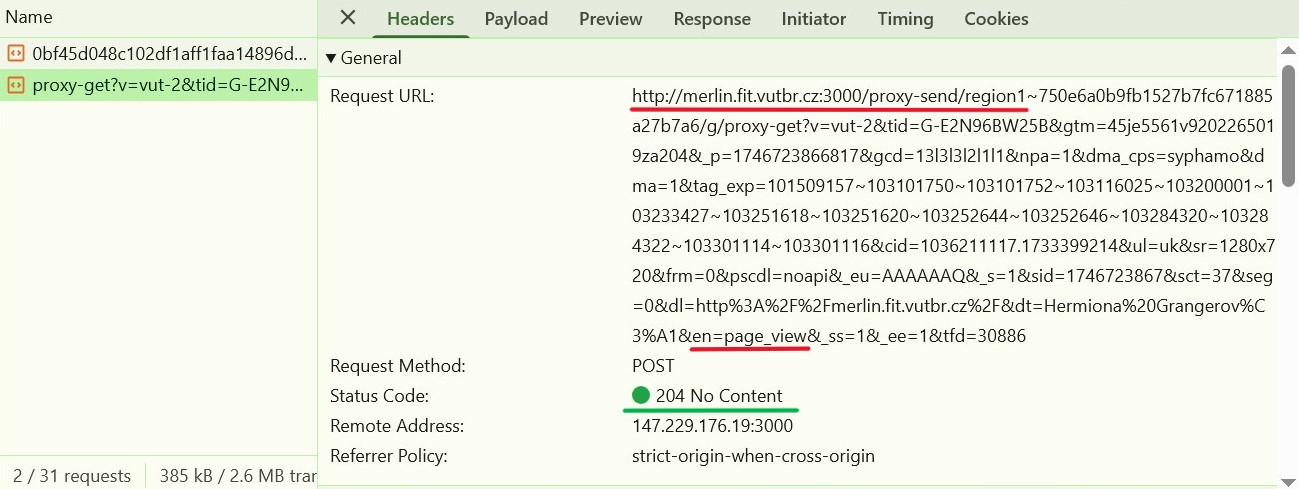
\includegraphics[width=1.0\textwidth]{obrazky-figures/reqTest2.jpg}
	\caption{Požadavek na odeslání události \texttt{page\_view}}
    \label{img:pageView}
\end{figure}

\begin{figure}[H]
	\centering
	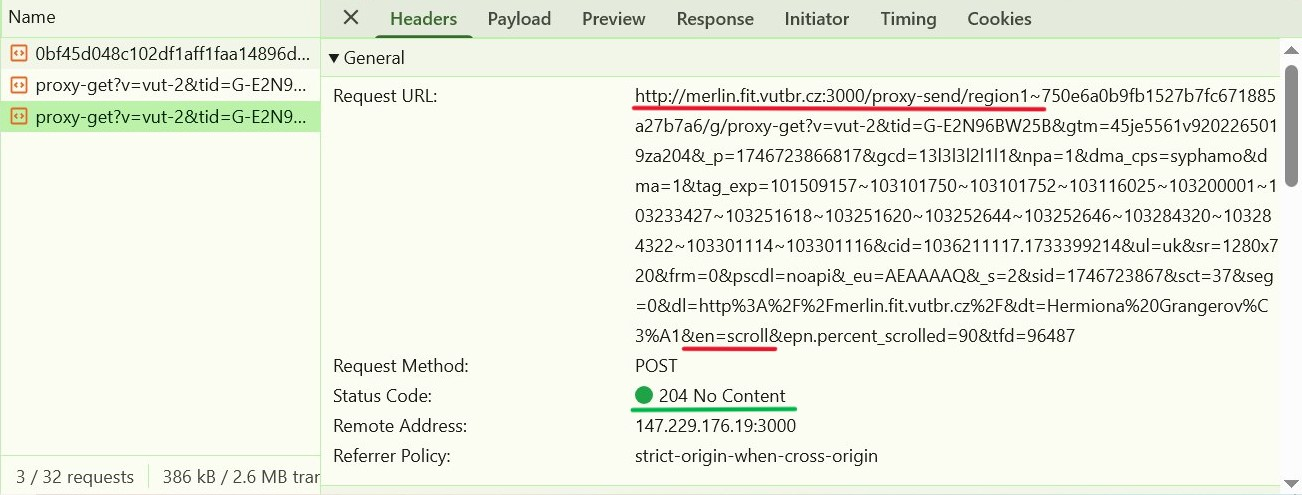
\includegraphics[width=1.0\textwidth]{obrazky-figures/reqTest3.jpg}
	\caption{Požadavek na odeslání události \texttt{scroll}}
    \label{img:scroll}
\end{figure}

Jak je vidět na snímcích obrazovky~\ref{img:pageView} a~\ref{img:scroll} získaných z z nástroje vývojáře sekce \texttt{Network}, server na oba požadavky odpověděl \texttt{204 No Content}, což je obecně přijímaný standard pro označení úspěšného přijetí požadavku bez vrácení dalšího obsahu v odpovědi. Poslední typ události nebylo možné zaznamenat nástrojem vývojáře, protože záložka byla zavřena, což automaticky ukončuje relaci nástroje vývojáře. Abych však zaznamenala i tento typ požadavku, přidala jsem dočasnou funkci pro zaznamenání přijatého maskovaného požadavku, který byl vrácen do původní podoby, a zaznamenání odpovědi cílového serveru na tento požadavek. Tímto způsobem jsem se ujistila, že proxy přijal a obnovil všechny tři typy požadavků a přesměroval je do Google Analytics.

\begin{figure}[H]
	\centering
	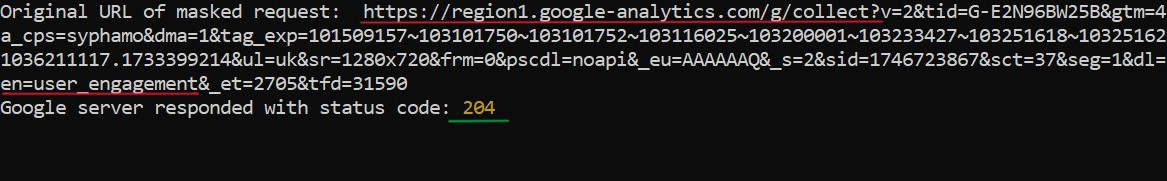
\includegraphics[width=1.0\textwidth]{obrazky-figures/reqTest4.jpg}
	\caption{Požadavek na odeslání události \texttt{user\_engagement}}
\end{figure}

Závěrečnou fází testování tohoto scénáře bylo ověření, že samotná služba Google Analytics rozpoznala a správně interpretovala přijaté požadavky. Za tímto účelem jsem se následující den po testu přihlásila do svého účtu Google Analytics a zkontrolovala souhrnné údaje o aktivitě uživatelů na mém webu. Byly tam jasně zaznamenány všechny tři události, které jsem na webu provedla: zobrazení stránky (\texttt{page\_view}), procházení stránky (\texttt{scroll}) a ukončení relace (\texttt{user\_engagement}). Všechny interakce s webem, které jsem provedla v tomto a předchozích testovacích scénářích, byly provedeny z jednoho zařízení a v jednom profilu prohlížeče. V rozhraní Google Analytics byly všechny tyto události spojeny, tj. byly identifikovány jako patřící jednomu uživateli. To konečně potvrdilo, že proxy server, který jsem implementovala, úspěšně splnil svou funkci -- obešel blokátor a umožnil analytickým skriptům vykonat svou práci na stránce uživatele.

\subsection*{Google Ads}
Pro ověření správného fungování remarketingu jsem použila svůj vlastní účet v Google Ads, v rámci kterého byl vygenerován identifikátor účtu. Tento identifikátor byl přidán do konfigurace základního {\it tagu} umístěného na mé univerzitní stránce. To znamená, že jsem nahradila ID Google Analytics, které bylo v {\it tagu}, ID Google Ads. Za účelem simulace reálného scénáře remarketingu jsem vytvořila nový segment publika, do kterého měli být přidáni všichni uživatelé, kteří navštíví uvedenou stránku. To odpovídá typickému a základnímu scénáři remarketingových skriptů, kdy se cílová skupina tvoří na základě chování uživatelů na webu. Algoritmus nastavení {\it tagu} pro remarketing se nelišil od jeho integrace pro službu Google Analytics. Hlavní změna se týkala identifikátoru produktu Google v konfiguraci {\it tagu}. Předpoklady testování byly stejné jako při testování Google Analytics. Otevřela jsem svou stránku v prohlížeči, ve kterém byl aktivován blokátor reklam uBlock Origin Lite v režimu úplného filtrování, a také byl otevřen nástroj pro vývojáře. Na stránce jsem neprováděla žádné další akce, simulovala jsem nejjednodušší návštěvu webového zdroje uživatelem.

V důsledku analýzy síťového provozu stránky bylo zaznamenáno úspěšné přijetí skriptu \texttt{gtag.js} prohlížečem a po jeho spuštění {\it tag} odeslal událost \texttt{page\_view}, která je standardní pro prohlížení stránky. Maskovaný požadavek byl odeslán proxy serveru a přesměrován na server Google Ads. V odpovědi cílový server odeslal status \texttt{200 OK}, což svědčí o úspěšném doručení a zpracování informací na straně Google Ads.

Během času vyhrazeného pro testování se segment publika v Google Ads nenaplnil uživateli. Místo toho se v rozhraní účtu zobrazilo upozornění, že pro aktivaci segmentu je nutné mít alespoň 1000 aktivních uživatelů. Takový provoz nebylo možné v rámci mého lokálního testování dosáhnout.  Navzdory tomu, obcházení blokátoru a přesměrování požadavků, jak jsem popsala výše, proběhlo úspěšně: {\it tag} byl aktivován, událost \texttt{page\_view} byla odeslána a služba Google Ads vrátila stavový kód \texttt{200}, který potvrzuje přijetí a zpracování požadavku. Ačkoli konečný cíl, tedy naplnění segmentu, nebyl dosažen, provedený test prokázal účinnost přístupu k maskování URL a přesměrování požadavků pomocí proxy, které jsem vytvořila.

Poslední scénář v rámci testování s různými službami Google předpokládal ověření fungování marketingového skriptu. Jak jsem však již popsala v sekci~\ref{sec:2:marketing}, pro realizaci marketingových cílů v rámci služby Google Ads není nutné implementovat žádný kód na vlastní webové stránce. Všechny klíčové procesy související se správou, nastavením a optimalizací marketingových kampaní se odehrávají v rámci účtu vytvořeného v Google Ads. To znamená, že na rozdíl od analytických a remarketingových scénářů nevyžadují marketingové skripty přímou interakci mezi stránkou a serverem Google. Jak jsem již popsala v sekci~\ref{sec:2:marketing}, data, která mohou být použita pro marketingové skripty, jako například shromážděné analytické informace nebo segmenty publika, jsou obvykle již zpracována a nacházejí se v produktech Google, například v přehledech Google Analytics nebo v sekci Správce publika v Google Ads. Vzhledem k výše uvedenému lze tedy dojít k závěru, že marketingové skripty nevytvářejí komunikaci mezi klientským prohlížečem a cílovým serverem, a proto nevyžadují maskování a přesměrování proxy serverem jako způsob obcházení blokátoru. 

\section{Testování s mezipamětí}
Tato sekce je věnována testování implementovaného proxy serveru v různých situacích souvisejících se stavem mezipaměti prohlížeče uživatele. Provedení testovacích scénářů souvisejících s mezipamětí umožňuje posoudit, jak stabilně program funguje v podmínkách reálného používání webu při první a opakované návštěvě stránky. To také umožňuje odhalit potenciální omezení proxy serveru související s chováním prohlížeče. 

V této sekci budou popsány dva nejtypičtější scénáře: 

\begin{enumerate}
    \item Prohlížeč s úplně vyčištěnou mezipamětí -- scénář, který odpovídá první návštěvě stránky uživatelem nebo jeho interakci s webem v anonymním režimu.
    \item Prohlížeč s uloženou mezipamětí po návštěvě stránky -- scénář, který simuluje opakovanou návštěvu stránky stejným uživatelem, když je v prohlížeči již uložena část zdrojů webu. 
\end{enumerate}

Tyto scénáře odpovídají reálným variantám chování uživatele a jeho prohlížeče a musí ukázat, že proxy je schopen plnit svou funkci v obou situacích, nezávisle na ukládání do mezipaměti na straně klienta.

\subsection*{Prohlížeč s úplně vyčištěnou mezipamětí}
Algoritmus prvního scénáře první návštěvy je stejný jako pro testování popsané výše v sekci~\ref{ch:6:testBlok}. Před zahájením testování: spustím proxy server na serveru \texttt{Merlin}, ručně vymažu mezipaměť prohlížeče, otevřu nástroj pro vývojáře a přejdu na odkaz proxy serveru. V této fázi bych chtěla poznamenat, že načítání stránky trvá o něco déle než obvykle, a to jak v tomto testu, tak ve všech předchozích. To je očekávané chování související s tím, že ve fázi získávání skriptu \texttt{gtag.js} proxy serverem program prochází celý seznam pravidel \texttt{EasyPrivacy} a maskuje nalezené shody ve skriptu. Tento algoritmus maskování vyžaduje optimalizaci, pokud bude můj proxy server implementován do skutečného komerčního projektu. Důvodem je netrpělivost uživatelů, kteří možná nepočkají na úplné načtení stránky a rozhodnou se ji opustit dříve, což je v rozporu se zájmy majitelů webových stránek, kteří potřebují co nejvíce přilákat zákazníky. 

Návratem k testování scénáře první návštěvy: výsledkem bylo  úspěšné načtení stránky, získání {\it tagu} skriptu ze serveru Google Tag Manager a jeho plné fungování na straně prohlížeče klienta. Proxy server tak prokázal stabilní a očekávané chování bez odchylek. 

\subsection*{Prohlížeč s uloženou mezipamětí po návštěvě stránky}
Druhý scénář byl proveden bezprostředně po skončení prvního, bez zavření stránky. Pro simulaci opakované návštěvy uživatele jsem znovu načítala webovou stránku, aniž bych cokoli měnila nebo dělala. V prvním scénáři tedy měl prohlížeč částečně uložit data stránky do mezipaměti, včetně skriptu \texttt{gtag.js}. Tento uložený keš byl použit při opětovném načtení stránky a skriptu \texttt{gtag.js}. Výsledek tohoto testu byl také pozitivní: stránka se načítala správně, několikrát rychleji než v předchozím scénáři, a proxy server zpracoval požadavky bez chyb nebo jakýchkoli odchylek v logice práce. To znamená, že implementovaný program pro přesměrování a maskování URL funguje stabilně i při opakovaném použití dat uložených v mezipaměti prohlížeče.

Pozornost je třeba věnovat jednomu architektonickému aspektu implementace proxy serveru. V době implementace se předpokládala, že proxy bude pracovat nepřetržitě, tj. spustí se jednou a bude pracovat paralelně s fungujícím webovým serverem. Právě proto jsou shody mezi původní URL a z ní vytvořeným hešem uloženy v globální mapě \texttt{urlMap}, která existuje v paměti pouze v rámci jednoho procesu serveru. To znamená, že v případě restartu proxy serveru bude předchozí obsah mapy ztracen. Pokud z nějakého důvodu je třeba proxy server zastavit, zejména v případě aktualizace nebo opravy chyb, \texttt{urlMap} ztratí potřebné shody a v případě, že uživatel po restartu proxy znovu vstoupí na web, program nebude schopen získat z maskovaných URL původní. K odstranění této slabiny je nutné implementovat mechanismus trvalého ukládání odpovídajících původních a hešovaných URL adres. Toho lze dosáhnout uložením URL mapy lokálně v souboru adresáře, kde se nachází proxy server, nebo uložením do databáze, která bude načtena při spuštění proxy serveru. Tento přístup zajistí stabilitu systému i po jeho restartu.

Kromě toho je důležité poznamenat, že mezi jednotlivými spuštěními proxy serveru je nutné odstranit soubor \texttt{gtag.js} ze složky \texttt{proxy-cache}, aby nový požadavek na jeho načtení vedl k získání původního skriptu ze serveru Google Tag Manager, což by spustilo mechanismus vyhledávání potenciálně blokovaných URL, jejich maskování a nové vyplnění globální mapy \texttt{urlMap} odpovídajících URL a jejich keše.

\chapter{Závěr}
\label{ch:7}
Cílem této práce bylo navrhnout a realizovat nástroj, který by byl schopen zajistit správné fungování analytických, marketingových a remarketingových skriptů i v situacích, kdy je na straně uživatele aktivován blokátor, který filtruje na základě seznamů blokovaných URL adres.

Za tímto účelem jsem v úvodní fázi práce prozkoumala a v kapitole~\ref{ch:2} popsala princip fungování a způsob použití analytických, marketingových a remarketingových skriptů, přičemž jsem jako příklad použila skripty poskytované platformami Google, jako jsou Google Analytics a Google Ads. Z tohoto důvodu jsem si vytvořila účet na obou službách Google, což mi umožnilo podrobněji prozkoumat fungování těchto platforem v praxi. Tyto znalosti a účty byly následně použity k testování funkčnosti vytvořeného nástroje v podmínkách blízkých reálným.

Následně v kapitole~\ref{ch:3} jsem seznámila čtenáře s riziky, kterým se mohou vystavit při surfování na internetu. Kromě toho jsem se seznámila s principy fungování blokátorů reklam, sledovacích trackerů a jiného nežádoucího obsahu, které fungují na základě filtračních seznamů. Jako konkrétní příklady jsem uvedla tři populární rozšíření prohlížečů, které plní roli podobných blokátorů. Mezi tyto příklady patří rozšíření uBlock Origin, jeho analog uBlock Origin Lite, Adblock Plus a Ghostery. Každé z těchto rozšíření jsem nainstalovala do svého prohlížeče Google Chrome, abych ukázala, jak konkrétně vypadají nastavení a dostupné režimy práce každého rozšíření z pohledu uživatelského rozhraní. 

Získána informace se stala základem pro vytvoření technického řešení popsaného v kapitole~\ref{ch:4}. Navrhla jsem vytvoření proxy serveru, který by fungoval jako prostředník mezi prohlížečem uživatele a externími servery. Hlavní myšlenka spočívala v zachycení požadavků, zpracování odpovědí a maskování potenciálně blokovaných URL adres ve skriptech a na HTML stránce takovým způsobem, aby se obešlo filtrování blokátorů na straně uživatele. V rámci kapitoly bylo popsáno princip fungování proxy serveru, stejně jako všechny hlavní fáze jeho interakce s prohlížečem klienta a externími servery.

Faktická realizace proxy serveru, popsaná v kapitole~\ref{ch:5}, se poněkud lišila od počátečního zámeru. Místo změny v konfigurace {\it tagu} cílového serveru na proxy server, aby mohl přijímat shromážděné údaje, byl v rámci proxy serveru implementován algoritmus, který maskuje v získaném skriptu \texttt{gtag.js} všechny potenciálně blokované URL adresy nebo jejich části. Podrobný popis procesu implementace a konečné verze proxy serveru je uveden v kapitole~\ref{ch:5}.

Závěrečnou fází práce bylo komplexní testování implementovaného proxy serveru s využitím mé stránky umístěné na univerzitním serveru Merlin. Pro rozsáhlé testování nástroje byly vytvořeny scénáře, které jsem rozdělila do třech skupin. V první skupině jsem testovala program s využitím různých rozšíření prohlížeče na straně uživatele, které fungují jako blokátory obsahu. Ve druhé skupině scénářů jsem se zaměřila na ověření interakce {\it tagu} s příslušnými platformami Google souvisejícími s marketingem, analytikou a remarketingem. Třetí a poslední skupina scénářů byla věnována modelování chování prohlížeče uživatele při první a opakované návštěvě stránky. Tímto způsobem jsem otestovala správnost obcházení různých blokátorů, úspěšnost přesměrování maskovaných požadavků, které by byly zpracovány cílovými servery Google, a stabilitu práce proxy serveru v podmínkách různých stavů uživatelského prohlížeče. Ve všech scénářích proxy server podle nastaveného algoritmu stabilně zpracovával požadavky a zajišťoval správnou interakci stránky s externími servery. I ve scénáři s testováním remarketingového publika navzdory tomu, že segment nebyl naplněn z důvodu nedostatečného počtu návštěvníků webu, což bylo způsobeno omezeným časem na testování a nemožností zajistit potřebný počet návštěvníků, a to minimálně 1000 uživatelů, proxy správně přesměroval potřebné požadavky a získal úspěšný stavový kód. 

V rámci dalšího vylepšování proxy serveru by bylo možné implementovat složitější a výkonnější parser pro zpracování seznamu filtrů EasyPrivacy. To by umožnilo pokrýt co největší počet URL adres, které podléhají blokování. Kromě toho by bylo možné optimalizovat algoritmus vyhledávání a maskování URL v skriptech typu \texttt{gtag.js}, aby se urychlil proces načítání stránky v prohlížeči uživatele  při jejích prvních návštěvách.

